%%!TEX encoding = UTF-8 Unicode

% Several lines in file have comments suggesting common packages for the
% typical thesis in informatics or electronics developed at UA
% uncomment/comment the lines as required for your work
% Before each optional line you will have a small comment

% According to UA rules, font size should range from 10 to 12pt.
\documentclass[11pt,a4paper,openright,twoside,onecolumn]{memoir}

\listfiles
\fixpdflayout

\usepackage[utf8]{inputenc}

% Select Computer Modern Typewritter (For bold ttfamily in listings)
\usepackage{lmodern}
% OR... Bera Mono
%\usepackage[scaled]{beramono} % TTT Font
%\usepackage{anyfontsize} % As the name says...

\usepackage[T1]{fontenc}

% Enable for for Overleaf support
\usepackage{ifthen}
\def\useoverleaf{1}  % change to non-zero (for instance, 1) to enable it

\makeatletter
\newcommand{\makecoverfile}[0]{%
  \immediate\write18{latexmk -pdf cover.tex}%
}
\makeatother

% For PDF merging
\usepackage{pdfpages}

% Set DPI to 300
\pdfpxdimen=\dimexpr 1in/300\relax

% Allow the use of a larger number of packages
\usepackage{morewrites} 

% For English and Portuguese languages
% Portuguese will be the default.
% Uncomment \setlanguage below to change it
\usepackage[english,portuguese]{babel}

% Uncomment to use a custom date format
%\usepackage{datetime}
%\newdateformat{thesisdate}{\monthname[\THEMONTH] \THEYEAR} % Month Year

% Make pdf look better
\usepackage{microtype} 

% Uncomment to enable floats on facing pages
%\usepackage{dpfloat}

% Side by side figures
% Eg. Fig 1a, Fig 1b
% originally:
% \usepackage[hang,small,bf]{caption}
\usepackage[small,bf]{caption}
%\let\tion\undefined
%\let\subfloat\undefined
\usepackage{subcaption}

%\RequirePackage{textcase}

% Dropped Caps
%\usepackage{lettrine}

% Configure Hyperlink color
% As a matter or style, you may use this to enable/disable color boxes on links
%\usepackage[breaklinks=true,colorlinks=false,linkcolor=blue]{hyperref}
% Or use the default values provided by the hyperref package
\usepackage[
hidelinks % added by vsantos
]{hyperref}

% Redefine section names according to your preference
%\def\sectionautorefname{Section}
%\def\chapterautorefname{Chapter}
%\def\figureautorefname{Figure}
%\def\listingautorefname{Listing}
%\def\tableautorefname{Table}

% Redefine code boxes
\ifthenelse{\equal{\useoverleaf}{0}}
{\usepackage[outputdir=build]{minted}}
{\usepackage{minted}}%

\addto\captionsportuguese{%
  \renewcommand\listingscaption{Código}
}
\fvset{fontsize=\footnotesize} % Make Code blocks smaller than text
\usepackage{csquotes}

% Add support for PDF Comments
\usepackage{comment}
\ifthenelse{\equal{\useoverleaf}{0}}
{\usepackage{pdfcomment}}{}
\usepackage{bookmark} % New Bookmarks

% For Multiple columns in Glossary
\usepackage{multicol}

% Add support for Math symbols
\usepackage{amsmath}
\usepackage{amssymb}

% Add support for graphics
\usepackage{graphicx}

% Add support for Colors
\usepackage{xcolor}

% Add support for the Euro symbol
\usepackage{eurosym}

% Add support for missingfigure and todo
% \usepackage{todonotes} % commented due to a conflict with pgf

% Setup bibliography with Biber using IEEE style for proper UTF-8 support
\usepackage[backend=biber, style=ieee, sorting=none, natbib=true, mincitenames=1, maxcitenames=2]{biblatex}
% in the proposal I used:
% \usepackage[backend=biber,style=numeric, sorting=none, maxnames=1,minnames=1]{biblatex}
\bibliography{bib/myrefs}

% Use acronyms
\usepackage[printonlyused]{acronym} % For acronyms

% Indenting the first paragraph after section start
\usepackage{indentfirst}

% For fixing listoflistings with memoir
\usepackage{xparse}

% Uncomment the next lines to enable chart support through pgf and tikz
% This may require you to install further packages in your Tex system
\usepackage[version=0.96]{pgf}
\usepackage{tikz}

% UML support
\usepackage{pgf-umlsd}

% Trees, Arrows, Mindmaps and other popular objects
\usetikzlibrary{arrows,shadows,trees,shapes,decorations,automata,backgrounds,petri,mindmap} % for pgf-umlsd

% Package to master SI units
\usepackage[detect-weight=true, binary-units=true]{siunitx}
% For Electric Circuits
%\sisetup{load-configurations = binary}

% Set Voltage direction accordingly
% Option : oldvoltagedirection,nooldvoltagedirection,RPvoltages,EFvoltages
% More information at: https://mirrors.ibiblio.org/CTAN/graphics/pgf/contrib/circuitikz/doc/circuitikzmanual.pdf
% By default this template is using the Old Voltage Direction
\usepackage[oldvoltagedirection,american,cuteinductors,smartlabels]{circuitikz}
\usetikzlibrary{calc}
\ctikzset{bipoles/thickness=1}
\ctikzset{bipoles/length=0.8cm}
\ctikzset{bipoles/diode/height=.375}
\ctikzset{bipoles/diode/width=.3}
\ctikzset{tripoles/thyristor/height=.8}
\ctikzset{tripoles/thyristor/width=1}
\ctikzset{bipoles/vsourceam/height/.initial=.7}
\ctikzset{bipoles/vsourceam/width/.initial=.7}
\tikzstyle{every node}=[font=\small]
\tikzstyle{every path}=[line width=0.8pt,line cap=round,line join=round]

% For inline TT text (e.g. code snippets)
\usepackage{verbatim}

% Frames around figures and allow force placement
\usepackage{float}

% Configure Float style
%\floatstyle{boxed}
%\restylefloat{table}
%\restylefloat{figure}
%\restylefloat{lstlisting}

% For test purposes you may use the lipsum package to create dummy text
\usepackage{lipsum} % REMOVE

% rotate images
\usepackage[figuresright]{rotating}

% combine rows
\usepackage{multirow}

% svg support
\usepackage[inkscapeformat=pdf]{svg}

%Keep floats inside section!
\usepackage[section]{placeins}
\let \oldsubsubsection \subsubsection
\renewcommand{\subsubsection}[2][]{
  \FloatBarrier
  \oldsubsubsection#1{#2}
}
\let \oldsubsection \subsection
\renewcommand{\subsection}[2][]{
  \FloatBarrier
  \oldsubsection#1{#2}
}
\let \oldsection \section
\renewcommand{\section}[2][]{
  \FloatBarrier
  \oldsection#1{#2}
}
\let \oldchapter \chapter
\renewcommand{\chapter}[2][]{
  \FloatBarrier
  \oldchapter#1{#2}
}


% Use the built-in division styling
\headstyles{memman}

% Include subsections in the TOC
\settocdepth{subsection}

% Numbering down to subsections as well
\setsecnumdepth{subsection}

% extra index for first lines
\makeindex[lines]

% Margins for University of Aveiro Thesis
\setlrmarginsandblock{3cm}{2.5cm}{*}
\setulmarginsandblock{3cm}{3cm}{*}
\checkandfixthelayout

% Or select your custom spacing to make any ajustment
%\addtolength{\parskip}{0.5\baselineskip}
\linespread{1.5}

% Some extra material added by vsantos
\usetikzlibrary{fit,positioning,shapes.geometric}
%

\newcommand\mainmatterWithoutReset
{\edef\temppagenumber{\arabic{page}}%
  \mainmatter
  \setcounter{page}{\temppagenumber}%
}


%%%%%%%%%%%%%%%%%%%%%%%%%%%%%%%%%%%%%%%%%%%%%%%%%%
% Document begins here
%%%%%%%%%%%%%%%%%%%%%%%%%%%%%%%%%%%%%%%%%%%%%%%%%%

\begin{document}
\ifthenelse{\equal{\useoverleaf}{0}}{}{\makecoverfile{}}%
\includepdf[pages=-]{cover.pdf}

% Uncomment to enable English
\selectlanguage{english}


% Front matter

%Custom Chapter style named `thesis`
\makechapterstyle{thesis}{% Based on ell
  \chapterstyle{default}
  \renewcommand*{\chapnumfont}{\normalfont\sffamily}
  \renewcommand*{\chaptitlefont}{\normalfont\Huge\sffamily}
  \settowidth{\chapindent}{\chapnumfont 111}
  \renewcommand*{\chapterheadstart}{\begingroup
    \vspace*{\beforechapskip}%
    \begin{adjustwidth}{}{-\chapindent}%
    \hrulefill
    \smash{\rule{0.4pt}{15mm}}
    \end{adjustwidth}\endgroup}
  \renewcommand*{\printchaptername}{}
  \renewcommand*{\chapternamenum}{}
  \renewcommand*{\printchapternum}{%
    \begin{adjustwidth}{}{-\chapindent}
    \hfill
    \raisebox{10mm}[0pt][0pt]{\fontsize{30}{25}\selectfont\chapnumfont \thechapter}%
                              \hspace*{1em}
    \end{adjustwidth}\vspace*{-3.0\onelineskip}}
  \renewcommand*{\printchaptertitle}[1]{%
    \vskip\onelineskip
    \raggedleft {\chaptitlefont ##1}\par\nobreak\vskip 4\onelineskip}}


% Select chapter style from existing or select custom
%\chapterstyle{thesis} % Others: dowding, demo2, dash, chappell, brotherton, bianchi, ger, madsen, tatcher, veelo,indexes)
% thesis can also be used as defined previously
% Check the memoir documentation for the available themes
% Default is veelo
\chapterstyle{veelo}
\makeoddfoot{plain}{}{\thepage}{} % Added by André Zúquete to fix a page numbering issue on the veelo chapter style


% If you feel adventurous you can also define all aspects of your theme
% Use either this input or the chapterstyle before
% % Rules
\newcommand{\thinRule}{\rule{\textwidth}{0.25pt}}

% Customize heading appearances
% Define styles
\newcommand{\partSize}{\Huge}
\newcommand{\partStyle}{\lsstyle\scshape}
\newcommand{\chapterSize}{\Huge}
\newcommand{\chapterStyle}{\lsstyle\scshape}
\newcommand{\chapterAfter}{}
\newcommand{\sectionSize}{\Large}
\newcommand{\sectionStyle}{\scshape\MakeTextLowercase}
\newcommand{\subsectionSize}{\large}
\newcommand{\subsectionStyle}{\scshape\MakeTextLowercase}
\newcommand{\subsubsectionSize}{\large}
\newcommand{\subsubsectionStyle}{\scshape\MakeTextLowercase}
\newlength{\partNumSizePt}
\setlength{\partNumSizePt}{60pt}
\newlength{\chapterNumSizePt}
\setlength{\chapterNumSizePt}{60pt}
\newcommand{\partNumSize}{%
  \fontsize{\partNumSizePt}{1.2\partNumSizePt}\selectfont%
}
\newcommand{\partNumStyle}{\partChapterNumColor}
\newcommand{\chapterNumSize}{%
  \fontsize{\chapterNumSizePt}{1.2\chapterNumSizePt}\selectfont%
}
\newcommand{\chapterNumStyle}{\partChapterNumColor}

% Customize parts
\renewcommand{\partnamefont}{\partSize\partStyle}
\renewcommand{\partnumfont}{\partNumSize\partNumStyle}
\renewcommand{\printpartname}{}
\renewcommand{\printparttitle}[1]{%
  \normalfont\normalcolor\partnamefont #1
}

% Customize chapters
\makeatletter
\setlength{\beforechapskip}{30pt}
\renewcommand*{\chapterheadstart}{\vspace*{\beforechapskip}}
\setlength{\afterchapskip}{3ex}
\setlength{\midchapskip}{3ex}
\renewcommand*{\chapnamefont}{%
  \Large\flushright\chapterStyle\partChapterNumColor%
}
\renewcommand*{\chapnumfont}{\chapterNumSize\chapterNumStyle}
\renewcommand*{\chaptitlefont}{%
  \normalfont\flushleft\normalcolor\chapterSize\chapterStyle%
}
\renewcommand*{\printchaptername}{%
  \chapnamefont\MakeTextLowercase{\@chapapp}%
}
\renewcommand*{\chapternamenum}{\quad}
\renewcommand*{\printchapternum}{%
%  \chapnumfont\textls[-75]{\classicstylenums{\thechapter}}%
 \chapnumfont\textls[-75]{\thechapter}%

}
\renewcommand*{\printchaptertitle}[1]{%
  \chaptitlefont #1
  \chapterAfter
}
\makeatother
% Customize sections and subsections
\setsecnumformat{\csname my#1\endcsname\quad}
\setsecheadstyle{\sectionSize\sectionStyle}
\newcommand{\mysection}{{\thesection}}
\setlength{\beforesecskip}{3em}


\setsubsecheadstyle{\subsectionSize\subsectionStyle}
\newcommand{\mysubsection}{{\normalfont\subsectionSize\thesubsection}}
\setlength{\beforesubsecskip}{3em}

\setsubsubsecheadstyle{\subsubsectionSize\subsubsectionStyle}
\newcommand{\mysubsubsection}{{\normalfont\subsubsectionSize\thesubsubsection}}
\setlength{\beforesubsubsecskip}{2em}

% Customize "Table of ..." appearance
% Customize headings
\newcommand{\renewPrintXTitle}[1]{%
  \renewcommand{#1}[1]{%
    \printchaptertitle{##1}%
  }%
}
\renewPrintXTitle{\printtoctitle}
\renewPrintXTitle{\printlottitle}
\renewPrintXTitle{\printloftitle}

% Customize ToC headings
\renewcommand{\cftpartfont}{\partChapterNumColor\partStyle}
\renewcommand{\cftchapterfont}{\chapterStyle}
\renewcommand{\cftsectionfont}{}
\renewcommand{\cftsubsectionfont}{}
\renewcommand{\cftfigurefont}{}
\renewcommand{\cfttablefont}{}
\newcommand{\cftlstlistingfont}{}

% Increase number width
\newlength{\cftNumWidthIncrease}
\setlength{\cftNumWidthIncrease}{0.25em}
\addtolength{\cftpartnumwidth}{\cftNumWidthIncrease}
\addtolength{\cftchapternumwidth}{\cftNumWidthIncrease}
\addtolength{\cftsectionindent}{\cftNumWidthIncrease}
\addtolength{\cftsubsectionindent}{\cftNumWidthIncrease}
% No leader dots
%\renewcommand*{\cftpartdotsep}{\cftnodots}
%\renewcommand*{\cftchapterdotsep}{\cftnodots}
%\renewcommand*{\cftsectiondotsep}{\cftnodots}
%\renewcommand*{\cftsubsectiondotsep}{\cftnodots}
%\renewcommand*{\cftfiguredotsep}{\cftnodots}
%\renewcommand*{\cfttabledotsep}{\cftnodots}
%\newcommand*{\cftlstlistingdotsep}{\cftnodots}
% Set page numbers immediately after entry text
\newcommand{\tocEntryPageSep}{\hspace{1em}}
\renewcommand{\cftpartleader}{\cftdotfill{\cftdotsep}}
%\renewcommand{\cftpartafterpnum}{\cftparfillskip}
%\renewcommand{\cftchapterleader}{\tocEntryPageSep}
\renewcommand{\cftchapterleader}{\cftdotfill{\cftdotsep}}
%\renewcommand{\cftchapterafterpnum}{\cftparfillskip}
\renewcommand{\cftsectionleader}{\cftdotfill{\cftdotsep}}
%\renewcommand{\cftsectionafterpnum}{\cftparfillskip}
\renewcommand{\cftsubsectionleader}{\cftdotfill{\cftdotsep}}
%\renewcommand{\cftsubsectionafterpnum}{\cftparfillskip}
\renewcommand{\cftfigureleader}{\cftdotfill{\cftdotsep}}
%\renewcommand{\cftfigureafterpnum}{\cftparfillskip}
\renewcommand{\cfttableleader}{\cftdotfill{\cftdotsep}}
%\renewcommand{\cfttableafterpnum}{\cftparfillskip}
\newcommand{\cftlstlistingleader}{\cftdotfill{\cftdotsep}}
%\newcommand{\cftlstlistingafterpnum}{\cftparfillskip}
% Customize page numbers
\newcommand{\tocPageStyle}{\tocPageColor}
\renewcommand{\cftpartpagefont}{\tocPageStyle}
\renewcommand{\cftchapterpagefont}{\tocPageStyle}
\renewcommand{\cftsectionpagefont}{\tocPageStyle}
\renewcommand{\cftsubsectionpagefont}{\tocPageStyle}
\renewcommand{\cftfigurepagefont}{\tocPageStyle}
\renewcommand{\cfttablepagefont}{\tocPageStyle}
\newcommand{\cftlstlistingpagefont}{\tocPageStyle}

% Abstract
% Remove indents around abstract text
\setlength{\absleftindent}{0pt}
\setlength{\absrightindent}{0pt}
% Change font size to conform with the rest of the document text
\renewcommand{\abstracttextfont}{\normalsize}

% Customize headers and footers including page numbers
\newcommand{\hfTextSize}{\footnotesize}
\newcommand{\headTextStyle}{\lsstyle\scshape\MakeTextLowercase}
\nouppercaseheads
\makeevenhead{headings}%
             {\hfTextSize\thepage}%
             {}%
             {\hfTextSize\headTextStyle\leftmark}
\makeevenhead{plain}%
             {\hfTextSize\thepage}%
             {}%
             {\hfTextSize\headTextStyle\leftmark}
\makeoddhead{headings}%
            {\hfTextSize\headTextStyle\rightmark}%
            {}%
            {\hfTextSize\thepage}
\makeoddhead{plain}%
            {\hfTextSize\headTextStyle\rightmark}%
            {}%
            {\hfTextSize\thepage}


% Customize captions
\newcommand{\captionSize}{\small}
\newcommand{\captionStyle}{\scshape}
\newcommand{\captionWidthRatio}{0.9}

\captionnamefont{\captionSize\captionStyle}
\captiontitlefont{\captionSize}
\captiondelim{ -- }
\captiontitlefinal{}
\changecaptionwidth
%\captionwidth{\captionWidthRatio\textwidth}

% Define colors
%\newcommand{\titleColor}{\color[rgb]{0.616, 0.0627, 0.176}}
\newcommand{\titleColor}{\color[rgb]{0,0,0}}

\newcommand{\partChapterNumColor}{\titleColor}
\newcommand{\dropCapColor}{\titleColor}
%\newcommand{\tocPageColor}{\color[rgb]{0.0980, 0.329, 0.651}}

\newcommand{\tocPageColor}{\color[rgb]{0, 0,0}}
\definecolor{shade0}{rgb}{1.0 , 1.0 , 1.0 }
\definecolor{shade1}{rgb}{0.9 , 0.9 , 0.9 }
\definecolor{shade2}{rgb}{0.8 , 0.8 , 0.8 }
\definecolor{shade3}{rgb}{0.65, 0.65, 0.65}
\definecolor{shade4}{rgb}{0.45, 0.45, 0.45}
\definecolor{shade5}{rgb}{0.0 , 0.0 , 0.0 }



%Exclude sub figures from List of Figures
%\captionsetup[subfloat]{list=no}

% Texts
\newenvironment{introduction}
{%
  \begin{minipage}{\textwidth}%
   \itshape%
}
{%
  \end{minipage}%
  \par\addvspace{2\baselineskip plus 0.2\baselineskip minus 0.2\baselineskip}%
}

% Select Page style
\pagestyle{plain}


\frontmatter

\tightlists
\midsloppy
\raggedbottom

\setcounter{tocdepth}{2} %subsections are added to the TOC
\setcounter{secnumdepth}{4} %subsubsections are numbered

% Initial document tables start here: TOC, LOF, LOT, Glossary
% Table of contents with slightly smaller font
\cleardoublepage
{\small\tableofcontents}

% List of figures with slightly smaller font
\cleardoublepage
{\small\listoffigures}

% List of tables with slightly smaller font
\cleardoublepage
{\small\listoftables}

% List of code snippets

% Fix for Listings with memoir

\RenewDocumentCommand \chapter { s O{#3} m }{%
  \FloatBarrier
  \IfValueTF{#1}  % if optional star is seen
    {\oldchapter*{#2}}
    {\oldchapter#1{#2}}
}

\renewcommand{\listingscaption}{Código}
\renewcommand{\listoflistingscaption}{Lista de Excertos de Código}
\cleardoublepage
{\small\listoflistings}
\addcontentsline{toc}{chapter}{\listoflistingscaption}

% Reset Chapters
\renewcommand{\chapter}[2][]{
  \FloatBarrier
  \oldchapter#1{#2}
}

% Print Glossary
{\small\chapter{Glossary}

\footnotesize
\SingleSpacing

\begin{multicols}{2}
\begin{acronym}[AAAAAA]

	\acro{h2o}[H2O]{Water}
	\acro{adsl}[ADSL]{Asymmetric Digital Subscriber Line}

\end{acronym}
\end{multicols}

}

%%%%%%%%%%%%%%%%%%%%%%%%%%%%%%%%%%%%%%%%%%%%%%%%%%%%%%%
% Main document starts here
%%%%%%%%%%%%%%%%%%%%%%%%%%%%%%%%%%%%%%%%%%%%%%%%%%%%%%%

\mainmatter

% Line spacing: 1.5 pt 
\OnehalfSpacing

%%%%%%%%%%%%%%%%%%%%%%%%%%%%%%%%%%%%%%%%%%%%%%%%%%%%%%%
% Start of Thesis text 
%%%%%%%%%%%%%%%%%%%%%%%%%%%%%%%%%%%%%%%%%%%%%%%%%%%%%%%

% Uncomment to add further chapters
%

\chapter{Example Chapter}
\label{chapter:example}

\begin{introduction}
A sort description of the chapter.

A memorable quote can also be used.
\end{introduction}



\section{Acrónimos}

Primeira e seguintes referências: \ac{h2o}, \ac{h2o}

Plural, acrónimo expandido e curto: \acp{h2o}, \acs{h2o}, \acl{h2o}

Com citação \footnote{Necessária entrada na bibliografia}: \ac{adsl}, \ac{adsl}


\section{Fontes}

\begin{itemize}
\item{\tiny Tiny}
\item{\scriptsize Scriptsize}
\item{\footnotesize Footnotes}
\item{\small Small}
\item{\normalsize Normal}
\item{\large large}
\item{\Large Large}
\item{\LARGE LARGE}
\item{\huge huge}
\item{\Huge Huge}
\end{itemize}

\section{Unidades}

Utilizando o pacote \verb|siunitx| é possível utilizar unidades do Sistema Internacional. Exemplo: a aceleração da gravidade é de \SI{9.8}{\metre\per\second\squared} e um ficheiro ocupa \SI{1}{\mebi\byte}. 

\section{Code Blocks}
\lipsum[5]

\begin{listing}
\begin{minted}{c}

#include <stdio.h>
#define N 10
/* Block
 * comment */
 
int main()
{
    int i;
 
    // Line comment.
    puts("Hello world!");
 
    for (i = 0; i < N; i++)
    {
        puts("LaTeX is also great for programmers!");
    }
 
    return 0;
}
\end{minted}
\caption{This is below the code.}
\label{lbl:snippet-test}
\end{listing}

\lipsum[5]

\chapter{Introduction}
\label{chapter:introduction}

\section{Background}

The Third Industrial Revolution was characterized by a focus on automating repetitive and heavy tasks on the assembly lines. Still, this created a problem: whenever the manufacturers needed the robots to work in a different assembly process, they needed to be reprogrammed by an expert. The Fourth Industrial Revolution, also known as Industry 4.0, refers to the current trend of the manufacturing sector to become more intelligent and achieve greater automation. This trend takes advantage of the recent developments in artificial intelligence, the Internet of Things, and autonomous robots to pave the way for more efficient and flexible production processes. With Industry 4.0, robots are expected to be more adaptable and perform more actions without constant explicit programming.

The concept of \acf{hrc} emerges as part of Industry 4.0 and involves the research of mechanisms that allow humans and robots to work together to achieve a shared goal. Some of the most relevant topics in recent research include collision avoidance and human-aware planning of robot motions. However, to achieve true collaboration, it is not enough to react to the partner’s movements and intentions, the robot must anticipate them.

\acf{ai} has significantly evolved in the last years. With the increase of computational power, \acf{ml}, a subset of \acs{ai}, has become an increasingly promising method to deal with complex data like images and text, heavily contributing to areas such as visual perception and speech recognition. \acl{ml} ’s ability to learn from data with minimal human intervention and understand new data it has never seen before makes it a prime candidate to solve many problems in robotics and \acs{hrc} in particular.

%This work attempts to use state-of-the-art \acs{ml} techniques to tackle the problem of action anticipation.

\section{Problem Description}

The concept of anticipation has been studied in several research fields, such as biology, psychology, and \acl{ai}. In general terms, anticipation is viewed as the impact of predictions on the current behavior of a system, be it natural or artificial. A prediction model provides information about the possible future state of the environment and/or system. This perspective of looking to the future is related to the purpose of incorporating that information into a decision-making or planning process. Accordingly, the system becomes anticipatory when it incorporates such a model and, simultaneously, when it uses the model to change its current behavior.

Over the last few decades, experimental evidences of the existence of anticipatory biological processes at different levels of organization have been reported \cite{Deans2021,Poli2010}. The ability to modify behavior in anticipation of future events offers an adaptive advantage to living organisms with an impact on behavioral execution and learning. Anticipation is also considered one of the required abilities of cognitive robots operating in dynamically changing environments. The role of anticipation is to connect the robot’s action in the present to its final goal, helping the design of robots with an increased level of autonomy and robustness.

The fundamental aspects of anticipation lie at the intersection of concepts such as time and information, involving abilities such as perception and prediction. The above definition of anticipation contains a temporal element that provides a key division between anticipatory and non-anticipatory robots. Anticipatory robots make decisions based on current states and predicted future states using predictive models of the environment. At the other extreme of the spectrum are the robots that live in the present based on the current state of the observed environment, which are usually called reactive robots (e.g., the Braintenberg’s vehicles \cite{Braitenberg1986}). However, the behavior of a purely reactive robot is limited by its temporal horizon since they have no memory of the past to build a model of the world. Most of the current robots present a behavior influenced either by the current perception as well as by the memory of past perceptions but still lacking a perspective of the future.

Information provides another defining aspect of anticipation since the prediction of a future state depends on sensory data. The challenge arises from the moment that an anticipatory system operates based on a potential future state (even before it occurs) that can only be inferred from past and current information. The inherent uncertainty associated with prediction process can be reduced through the acquisition of information, namely by using different sensory modalities. In this context, sensory fusion is a process often adopted to merge data from multiple sensors such that to reduce the amount of uncertainty that may be involved to produce more reliable knowledge about the future.

The nature of anticipation and the mechanisms that support it are considered open questions in \acs{ai} and robotics. Current research addresses fundamental questions such as: in which situations is anticipation useful? How can anticipatory processes be modeled and implemented in robotic systems? What are the impacts that may result from an anticipatory behavior? In the context of this dissertation proposal, we consider anticipation as a combination of prediction and decision-making, as illustrated by the blocks diagram in Fig.~\ref{fig:anticipatorysystem}. The prediction model offers the possibility of incorporating action selection in their planning through a decision-making block, while the planning module relates to the robot’s actions. These modules can be developed separately, or an end-to-end learning technique could be used where the model learns the different parts from the perception to the feedback control. 

\begin{figure}[H]%[!ht]
    \centering
    % Block of tikz code to draw the image of the Anticipatory System.
% Adapt at will.
% vsantos, 2023

\definecolor{colA}{HTML}{2a6099}
\definecolor{colB}{HTML}{729fcf}
\tikzset{
	myB/.style= %main block style
	{
		fill=colA,text=white, %comment this...
        %draw,  %...and uncomment this for a simpler diagram
		font=\sffamily,
		align=center,
		minimum height=1.5cm,
		text width=1.75cm,
		inner sep=2pt,
	},
	myT/.style= %the black triangle
	{
		isosceles triangle,
		fill=black,
		minimum height=8pt,
		isosceles triangle apex angle=140,
		anchor=apex,
        inner sep=1pt,
	},	
}

\def\nyDist{2.25cm}  %block separation
\pgfdeclarelayer{background layer}
\pgfsetlayers{background layer,main}
%Now the actual drawing
\begin{tikzpicture}[node distance=\nyDist]
\node [myB]              (per){Perception};
\node [myB,right of=per] (PM) {Prediction model};
\node [myB,right of=PM]  (DM) {Decision making};
\node [myB,right of=DM]  (MP) {Motion Planning};
\node [myB,right of=MP]  (FC) {Feedback Control};

\node [myB,below of=per] (per2) {Perception};
\node [myB, inner sep=0,
	fit={(PM) (MP)},
	yshift=-\nyDist,
	text depth=1.5em, %forced adjustment :-(
] (EEL) {End-to-end learning};
\node [myB,below of=FC] (FC2) {Feedback Control};

%Place all triangles with a loop ;-)
%Each triangle has a node name T1, T2, etc...
\foreach \NN [count=\i] in {PM,DM,MP,FC,EEL,FC2}
	\node [myT,at=(\NN.west)] (T\i) {};

%some tweaks to have the anticipatory layer well placed
\begin{pgfonlayer}{background layer}
\node [
	draw=colA,
	dotted,
	thick,
	fill=colB,
	fit=(PM.north west) (DM.south east),
	inner ysep=1em,
    yshift=0.5em,
	label={[anchor=north,font=\sffamily]north:Anticipatory layer}
	] (AL) {};
\end{pgfonlayer}

%Two auxiliary points to aid further
\coordinate (midL) at ($(per.west)!0.5!(per2.west)$);
\coordinate (midR) at ($(FC.east)!0.5!(FC2.east)$);

% The nodes at the extremes and the lines connecting them to the main blocks
\if{0}
\node [left of=midL,xshift=1cm,text width=1cm,font=\sffamily] (SI) {Sensor input};
\draw (SI) -- ([xshift=-10pt]midL) |- (per.west);
\draw (SI) -- ([xshift=-10pt]midL) |- (per2.west);

\node [right of=midR,xshift=-1cm,text width=1.25cm,font=\sffamily] (CO) {Control output};
\draw (CO) -- ([xshift=10pt]midR) |- (FC.east);
\draw (CO) -- ([xshift=10pt]midR) |- (FC2.east);
\fi

\node [left of=midL,xshift=1cm,text width=1cm,font=\sffamily] (SI) {Sensor input};
\draw (SI) |- (per.west);
\draw (SI) |- (per2.west);

\node [right of=midR,xshift=-1cm,text width=1.25cm,font=\sffamily] (CO) {Control output};
\draw (CO) |- (FC.east);
\draw (CO) |- (FC2.east);

\end{tikzpicture}
    \caption{Functional blocks of an anticipatory robotic system considering two alternative approaches: modules developed separately vs end-to-end learning.}
    \label{fig:anticipatorysystem}
\end{figure}

There are different situations in which an anticipatory response seems to be an essential ability for effective robot behavior. In an attempt to distinguish different types of anticipatory behaviors, three contexts in which a robot can operate are categorized below and the respective task requirements are presented as follows:

\begin{itemize}

\item \textbf{Time synchronization}. The interception of moving objects is central to several benchmark robotic tasks such as ball-catching and playing table tennis \cite{Carneiro2021, Wang2017}. These tasks are challenging due to the demanding spatial–temporal constraints, which require continuous coordination between visual, planning and control systems. On the one hand, frequent repredictions of the target location are required as new observations become available. On the other hand, this progressive refinement imposes an online re-planning of robot motion such that the goal is achieved in time.

\item \textbf{Preventive safety}. Systems that manage risk require some form of anticipatory mechanism such that the robot can adapt its behavior when an undesired situation occurs. Autonomous driving is an example of how predicting future events and reacting properly are important abilities to mitigate risk. Modeling behavior and predicting the future intentions of pedestrians are core elements to ensure that the driver stops the car safely or avoids the pedestrian in time.

\item \textbf{Coordinate joint activities in \acf{hri}}. Humans have the ability to coordinate their actions when carrying out joint tasks with other partners (\textcite{Sebanz2006,Hoffman2007}). In the same line of thought, anticipation can enhance the ability of a robot in its interaction with a human partner by predicting their actions (or intentions) before selecting its own action plan. In collaborative contexts such as those that occur during manufacturing or assembly tasks, the main challenge is combining anticipation and planning in a context of high uncertainty due to the variability of human behavior in complex industrial environments. Anticipation seems to have a significant potential for a more fluid and natural interaction with an impact on safety and cycle time.

\end{itemize}

This dissertation aims at the development of an anticipatory system that allows to enhance human-robot collaboration in industrial settings under the AUGMANITY mobilizing project\footnote{AUGMANITY website: \url{https://www.augmanity.pt}}. The collaborative scenario will be one in which the robot observes the actions of the human operator, makes predictions about the human’s intention and reacts accordingly by either waiting for more observations or executing a physical action. Fig.~\ref{fig:usecase} illustrates the real workstation where the structure of a gas boiler for water heating is manually assembled. The collaborative robot’s main function will be to assist with the assembly task by placing the parts in the jig while coordinating its actions with those of the human
operator who is focused on the riveting process. 

\begin{figure}[H]
\centerline{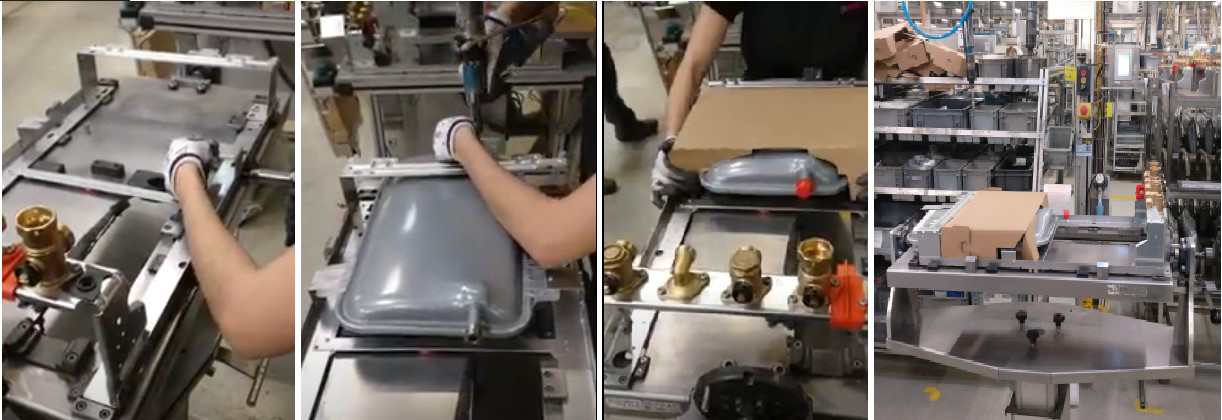
\includegraphics[width=6in]{figs/usecase.png}}
\caption{Different views of the current workstation used for the manual assemblage of the structure of a gas boiler for water heating.}
\label{fig:usecase}
\end{figure}

\section{Objectives}

\textcolor{red}{(taken from chapter 5 from proposal)}

\begin{enumerate}
    \item \textbf{Overview of the Experimental Setup}. Familiarization with the robot and tools that will be used throughout the dissertation.

    \item \textbf{Development of Action Anticipation Models}. To formally define how to anticipate an action in the context of the collaborative task under study using RGB-D images as input. \acs{ml} models, such as \acfp{rnn}, are at the forefront of the algorithms to explore.
    
    \item \textbf{Development of an Anticipatory Controller}. To develop robot controllers that consider the human partner's movements and intentions and use these inferences to make appropriate decisions during the execution of a sequential assembly task.

    \item \textbf{Metrics and performance evaluation}. To provide performance metrics used to evaluate the action anticipation models and the add-value of the anticipatory controller (e.g., in terms of cycle time).
    
    \item \textbf{Thesis Writing}. Writing the master dissertation and other detailed documentation.
\end{enumerate}

\section{Document Structure}

The remainder of the document is organized into five chapters. Chapter $ref{chapter:state_of_the_art}$ contains background material about anticipation, \acl{ml} and collaborative robotics and a review of previous work on Action Anticipation in \acs{hrc} including sensors and methods. Chapter $ref{chapter:tools_review}$ reviews tools that can be useful in the future implementation. Chapter $ref{chapter:work_progress}$ describes the progress made in the first semester. Chapter $ref{chapter:planning}$ portrays the planning of the second semester work and illustrates its calendarization. Chapter $ref{chapter:conclusion}$ concludes the document by restating the objectives of the work and the plan to achieve them.

\chapter{State of the Art}
\label{chapter:state_of_the_art}

This chapter starts by covering background concepts about anticipation in biology, \acl{ml} and collaborative robotics and then reviews previous work related to the dissertation theme, including sensors and methods.

\section{Background Material}

\subsection{Anticipation in Biology}

Anticipation is a research topic in many areas, such as biology, brain studies, psychology, social sciences, artificial intelligence, and engineering. One of the most cited definitions in the last decades and across the various fields is Rosen's \cite{Rosen1985}:

\begin{displayquote}
An anticipatory system is a system containing a predictive model of itself and/or its environment, which allows it to change state at an instant in accord with the model's predictions pertaining to a later instant.
\end{displayquote}

In the field of biology, \textcite{Louie2010} claims that \textquote{Much, if not most, biological behavior is model-based ...} with the referred models being the \textquote{... internal predictive models of themselves and their environments ...}. \textcite{Poli2010} further claims that \textquote{... given that anticipatory behavior dramatically enhances the chances of survival, evolution itself may have found how to give anticipatory capacities to organisms, or to at least some of them.}. For example, we can consider an animal predicting that it will be attacked by its predator and dodging said attack to survive.

In the case of humans, \textcite{ Louie2010} also stated, \textquote{We typically decide what to do now in terms of what we perceive will be the consequences of our action at some later time.} alluding to our anticipatory behavior. Therefore, human actions can result from reactive behavior when they are based on the past, from anticipatory behavior when they are based on predictions of the future, or from a mix of both.

In particular, sports is a field where, according to \textcite{Smith2016}, \textquote{Proficiency in action anticipation is relevant in many performance contexts such as anticipating the direction of a shot (in soccer, hockey, tennis, volleyball, badminton, etc.), the deceptive movement of an opponent (in soccer, basketball, rugby, football, boxing, etc.), or the movement of a partner (in figure skating, dancing, etc.).}.

\subsection{\acf{ml}}

\acl{ml} algorithms have been increasingly more common in the last years due to, for example, their ability to deal with multidimensional data. These algorithms can automatically learn from data and make predictions or decisions, which makes them a prime candidate to use in the context of human action anticipation in collaborative environments. The most common strategies in \acs{ml} are Supervised Learning, Unsupervised Learning, and Reinforcement Learning. \if{0}As we can see in Fig.~\ref{machinelearning} obtained from a review article about HRC in general, supervised learning and reinforcement learning are dominant in this area, with composite solutions surpassing unsupervised learning in the most recent year showed.

\begin{figure}[H]
\centerline{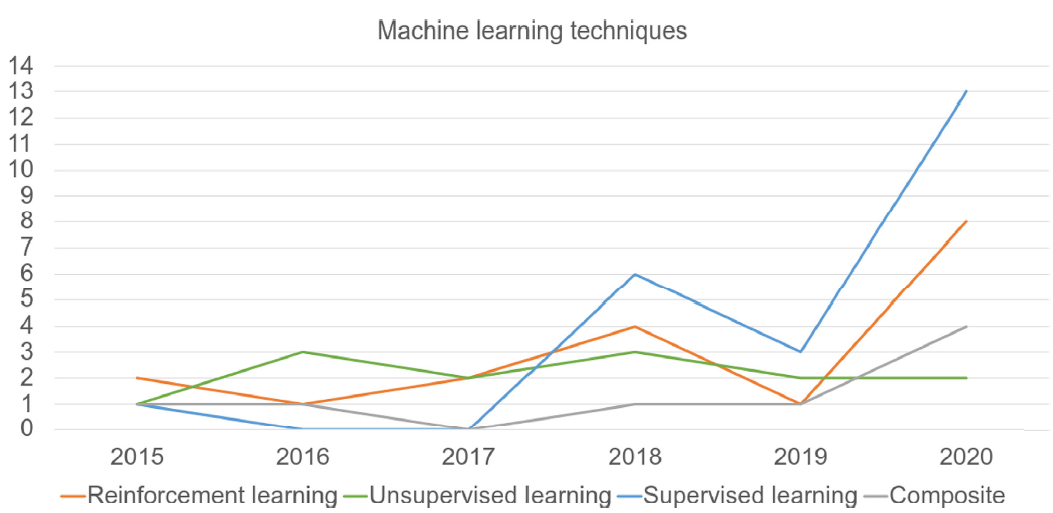
\includegraphics[width=6in]{figs/machinelearning.PNG}}
\caption{Number of articles relevant to the HRC review from each machine learning technique throughout the years\cite{Semeraro2023}}
\label{machinelearning}
\end{figure}
\fi

\subsubsection{Supervised Learning}

In Supervised Learning, the models are trained using a dataset of labeled data. According to \textcite{Sarker2021}, these models must generalize the knowledge from the dataset's input-output pairs to correctly deal with a new input they have never seen before. The models from this group are further divided into classification, where the new input is assigned a discrete output class, and Regression, where it is returned a real number from the continuous output space. Currently, \acs{rnn}s and \acs{cnn}s are two of the most common classification approaches.

A \acf{rnn} is a type of neural network where the output of each time step is fed back into the input at the next time step, allowing the network to remember and incorporate information from previous time steps into its processing of current and future data. This characteristic makes \acp{rnn} particularly well-suited to processing sequential data, such as text, speech, or time series data which require context or temporal dependencies. In particular, according to \cite{lstm_advantages}, \acf{lstm} is an \acs{rnn} with a more complex architecture that gives it an improved ability to backpropagate the error, making it better to train a model that classifies sequences with several time steps.

A \acf{cnn} is a type of neural network made up of several convolutional layers which apply a sliding filter over the input reducing its dimension and obtaining its features. Typically, these layers are followed by one or more fully connected layers that perform the prediction using the mentioned features. This architecture makes \acp{cnn} an excellent choice to deal with data in a matrix structure such as an image because this input is too massive for manual feature engineering.

In Supervised Learning, transfer learning is a technique that makes use of a trained external model. Depending on the goal of its use, these models can be entirely or partially used; optionally, they can also be trained partially or fully. A common use case for this technique is when a small dataset of images is used to obtain a classifier, and a standard model cannot generalize from that reduced amount of data. In this case, a model such as VGG-16 and ResNet-50 can be used partially to extract the features with one or more fully connected layers in the end, to perform the desired classification from those features.

\subsubsection{Unsupervised Learning}

%You say too little on this. Could you say more, or perhaps complement with an example?

In Unsupervised Learning, the datasets involved have no labels. According to \textcite{Sarker2021}, these algorithms aim to find patterns and structure in the data. This makes them valuable in tasks such as clustering based on common characteristics, density estimation, identifying anomalies and outliers, dimensionality reduction, feature learning and finding association rules.

Clustering is a technique used to create groups of points representing instances of the dataset to discover relevant trends or patterns. K-means clustering is one of the most common and simple clustering algorithms. It starts by creating $k$ random centroids and assigns each instance of the data to the closest centroid by squared distance. This process can be repeated to achieve better results. This algorithm works well when the points from different sets are considerably separated from each other.

Dimensionality reduction is a technique that aims to reduce the number of features by selecting a subset of the original ones using algorithms such as Chi-squared test or extracting new features from the originals using algorithms such as Principal Component Analysis (PCA).

%\textcolor{red}{Association Rule Learning is another possible example}

\subsubsection{\acf{rl}}

\acl{rl} is different from the previous approaches because it does not need a dataset. According to \textcite{Alom2019}, the agent learns how to act in an unknown environment by interacting with it. After the agent's action, the environment returns an observation and a certain reward to the agent depending on the quality of the action. The agent uses the reward to update its internal model named policy improving its future performance and the cycle repeats, as shown in Fig.~\ref{rl_diagram}. This type of learning by trial and error has a certain resemblance to how humans gain knowledge, and it is useful when there is a need for an agent to make decisions in an environment that has considerable complexity, such as controlling a robot or playing a game.

\begin{figure}[h]
\centering
%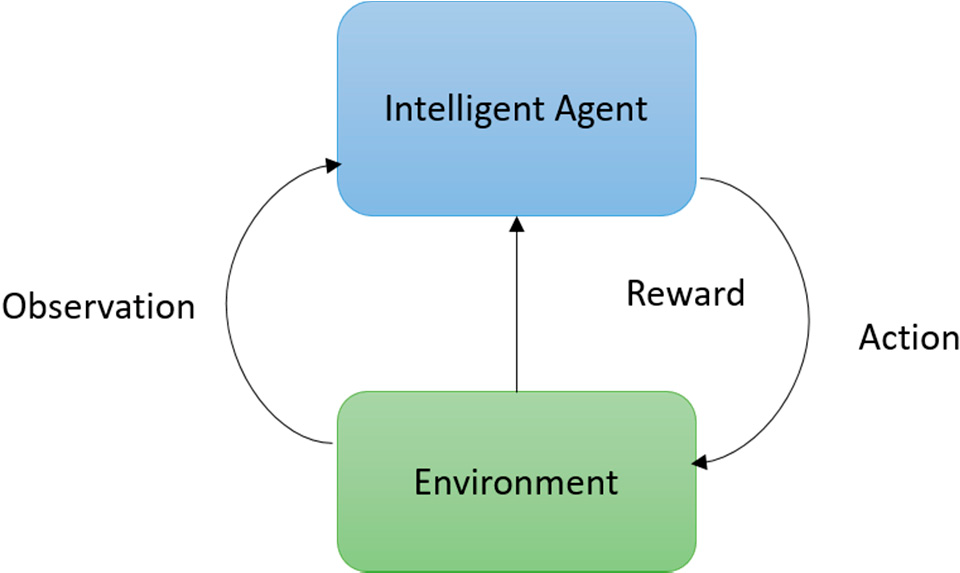
\includegraphics[width=7cm]{figs/rl_diagram.png}
%Alternative in tikz :-) vsantos
\begin{tikzpicture}[minimum height=1.5cm, text width=2cm, align=center,rounded corners,node distance=2.5cm]
\node [fill=blue!30] (IA) {Intelligent Agent};
\node [fill=green!40,below of=IA] (Env) {Environment};
\draw [->,>=stealth](Env) -- node [midway,right,xshift=-10pt] {Reward} (IA);
\draw [>=stealth] (IA.east) edge[->, in=0,out=0] node [midway,right,xshift=-10pt] {Action} (Env.east);
\draw [>=stealth] (Env.west) edge[->,in=180,out=180] node [midway,left] {Observation} (IA.west);
\end{tikzpicture}
%End of alternative -- vsantos
\caption[Interactions between the Agent and the Environment in \acs{rl}]{Interactions between the Agent and the Environment in \acs{rl} \cite{Alom2019}}
\label{rl_diagram}
\end{figure}

In the workflow of \acl{rl}, the agent must associate an observation to an environment state. This is a simple process in a small discrete environment since there are fewer states. However, if the environment has many variables or it is not discrete then it becomes challenging to associate states with an observation. In these cases, it is necessary to use deep \acl{rl}, which is able to extract the relevant information from the observation and use it to associate the observation with a state.

Given that to train a \acl{rl} model, it is necessary for the agent to interact with the environment thousands of times, this process ends up needing a simulator. According to \textcite{Li2023}, one of the major challenges in \acs{rl} is transferring the knowledge learned in the simulator to a real-life environment. There may be a gap between the real and the simulated environment because the real world has more or less observable variables causing a drop in performance. \textcite{Ahmed2020} also claims that this may be due to an incorrect design of the reward function leading to over-fitting and sub-optimal policies.

\subsection{Collaborative Robotics}
\label{subsection:collaborative_robotics}

\acf{hrc} consists of robots and humans working in the same workspace towards a common goal. Classical industrial robots are usually automated to perform repetitive tasks that require high physical strength. On the other hand, tasks that require cognitive knowledge, flexibility, and precision are better suited for humans, even if they are physically weaker. \acs{hrc} aims to take advantage of both of their strengths and complement each others' weaknesses to increase manufacturing efficiency.

In a \acs{hrc} scenario, robots need to be different from the traditional ones, given that they will work in the same workspace as humans. According to \textcite{Castro2021}, \textquote{Collaborative robots need to be endowed with a set of abilities that enable them to act in close contact with humans, such as sensing, reasoning, and learning. In turn, the human must be placed at the centre of a careful design where safety aspects and intuitive physical interaction need to be addressed as well.}. In \cite{CobotsWW}, it is stated that nowadays, collaborative robots are developed to be compact, easy to install and program, flexible, mobile, consistent and precise. Additionally, they positively impact employees since they are responsible for monotonous and dangerous actions and reduce the production cost for the company.

\subsubsection{Human-Robot Communication}

Humans and robots can communicate through several methods, which can be direct such as using a console or a remote, or indirect, resulting from data captured from sensors. Based on \cite{Castro2021, Mukherjee2022, Semeraro2023,}, the main methods for indirect communication can be seen in the diagram in Fig.~\ref{interaction} and can be described as follows:

\begin{figure}[ht]
\centering
%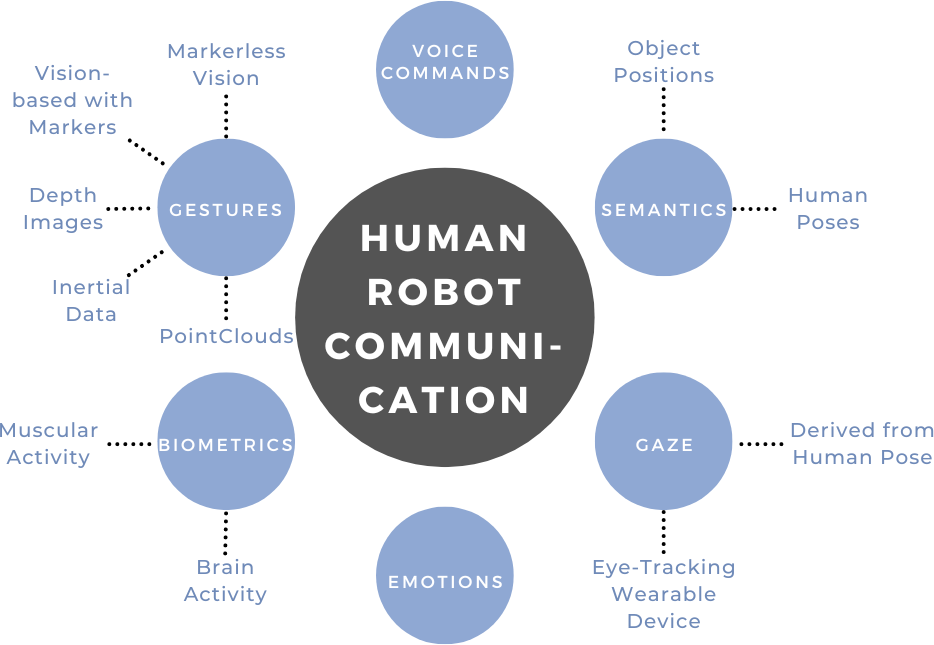
\includegraphics[width=5.5in]{figs/interaction.png}
%% by vsantos, 23 Mar 2023
\definecolor{vColorA}{HTML}{545454}
\definecolor{vColorB}{HTML}{8fa8d3}
\begin{tikzpicture}[scale=0.75,transform shape,
	mindmap,
	grow cyclic,
	every node/.append style={
				concept,
				inner sep=0pt,
				concept color=vColorB,
    font=\sffamily,
				}, %this is appended to all local props!
	concept color=vColorB,
	text=white,
%	font=\sffamily\bfseries\Large,
	level 1/.append style={
%							level distance=5cm,
%							sibling angle=60,
	%						font=\sffamily,
%							concept color=vColorB,
							},
	level 2/.append style={
%							level distance=2.75cm,
							sibling angle=45,
%							font=\small \sffamily,
							text=black,
%							concept color=white,
						  },
]

\node[] (HRC) at (0,0){\large\bfseries HUMAN ROBOT COMMUNICATION}
	[counterclockwise from = -30]
child[]
{
	node[](Gaze){GAZE}
	[clockwise from = 0]
	child{node[](dhp){Derived from human pose}}
	child{node[](eye) {Eye-tracking Wearable Device}}
}
child[]
{
	node [] (Semantics) {SEMANTICS}
	[counterclockwise from = 0]
	child{node[](hp){Human Poses}}
	child{node[](op) {Object Positions}}
}
child[]
{
	node [] (VoiceCommands) {VOICE COMMANDS}
}
child[]
{
	node []  (Gestures) {GESTURES}
		[counterclockwise from = 60] %[grow=180]
		child{node[](mv){Markerless Vision}}
		child{node[](vbm) {Vision based with Markers}}
		child{node[](di) {Depth Images}}
		child{node[](id) {Inertial Data}}	
		child{node[](pc) {Point clouds}}	
}
child[]
{
	node [] (Biometrics) {BIO-METRICS}
		[counterclockwise from = 180]
		child{node[](ma){Muscular Activity}}
		child{node[](ba) {Brain Activity}}	
}
child[]
{
	node [] (Emotions) {EMOTIONS}
}
;

\end{tikzpicture} %an optional representation :-) %vs

\caption{Data sources common in \acl{hrc}}
\label{interaction}
\end{figure}

\begin{itemize}
\item \textbf{Gestures}: these are one of the main ways humans communicate, whether through simple movements or formal sign language. In the literature about \acs{hrc}, gestures can also commonly be found since they have the advantage of resisting ambient noise. Usually, gestures are captured with vision-based methods with either an RGB or RGB-D camera, so there is no need for unnatural movements. With vision, it is possible to include markers, but these may lead to occlusions and hinder the worker's movements. Consequently, there is also work in the literature that uses markerless vision to allow more unrestricted movements. Another way to capture the movements of the human worker would be to use wearable inertial sensors, which contain accelerometers and gyroscopes, but, once again, wearables can hinder the worker's movements. Finally, capturing point clouds using a LIDAR presents another possibility of capturing gestures without restricting the worker's motion.

% Do you mean spoken language by means of sound or written or typed text, or can it be more than this?

\item \textbf{Voice Commands}: Talking is the most intuitive way for humans to communicate with each other. The advances in voice recognition and natural language processing make this a possible communication solution with robots. However, despite being intuitive, simple, effective, and even robust against lighting variations, when it comes to an industrial setting that contains significant sound noise, it becomes less valuable than the alternatives.

\item \textbf{Semantics}: semantic information about the objects can also help the global workflow. For example, suppose the robot is trained to recognize certain features in objects related to how it can pick them up. In this case, the robot can pick up a new object it has never seen before if it has a similar structure. Human actions can also be represented semantically by obtaining the poses of the human as a specific set of limbs, even if only partially. During action recognition, this can be used to know which objects the worker can interact with. Having semantic information about the pose of the human body also helps in the path-planning phase of the robot since it can use this information to avoid the worker and prevent collisions.

\item \textbf{Gaze}: this can be used to determine where the user's attention resides, giving a considerable amount of information that can trigger some action. There are two options to obtain the user's gaze. Wearable sensors can provide better results but are expensive and intrusive. On the other hand, algorithms that detect head pose and assume the gaze from it can also be used, which is a cheaper and non-intrusive solution.

\item \textbf{Emotions}: although this is a relatively new idea, some applications analyze the user's emotions from his facial expressions to have even more information in the algorithms.

\item \textbf{Biometrics}: \acf{emg} sensors can measure electrical signals generated by muscle contractions, while electroencephalography (EEG) signals are commonly used in brain-computer interfaces (BCIs). %\textcolor{blue}{And why not heart beat, breath, ...?}

\end{itemize}

\subsubsection{Safety}

Safety is one of the most critical topics in collaborative robotics and the first step toward establishing a collaborative environment. According to \cite{CobotsWW}, collaborative robots are able to safely work with people because they have sensitive sensors that can detect the human interrupting them, causing them to stop their actions, while traditional robots would potentially injure the worker. However, given that there are tasks that require the robot to move very close to the worker, some norms were implemented: ISO 10218-1 and 10218-2. From these two standards, \textcite{Castro2021} and \textcite{Villani2018} describe the four criteria from which at least one must be met as:
\begin{enumerate}
  \item \textbf{Safety-rated monitored stop}: when a human enters the cobot's workspace, it completely stops;
  \item \textbf{Hand guiding}: when an operator manually moves the cobot, it is compliant;
  \item \textbf{Speed and separation monitoring}: as the human moves closer to the cobot, it becomes gradually slower;
  \item \textbf{Power and force limiting}: the cobot has its operation restricted in terms of force and torque.
\end{enumerate}

\begin{figure}[ht]
\centerline{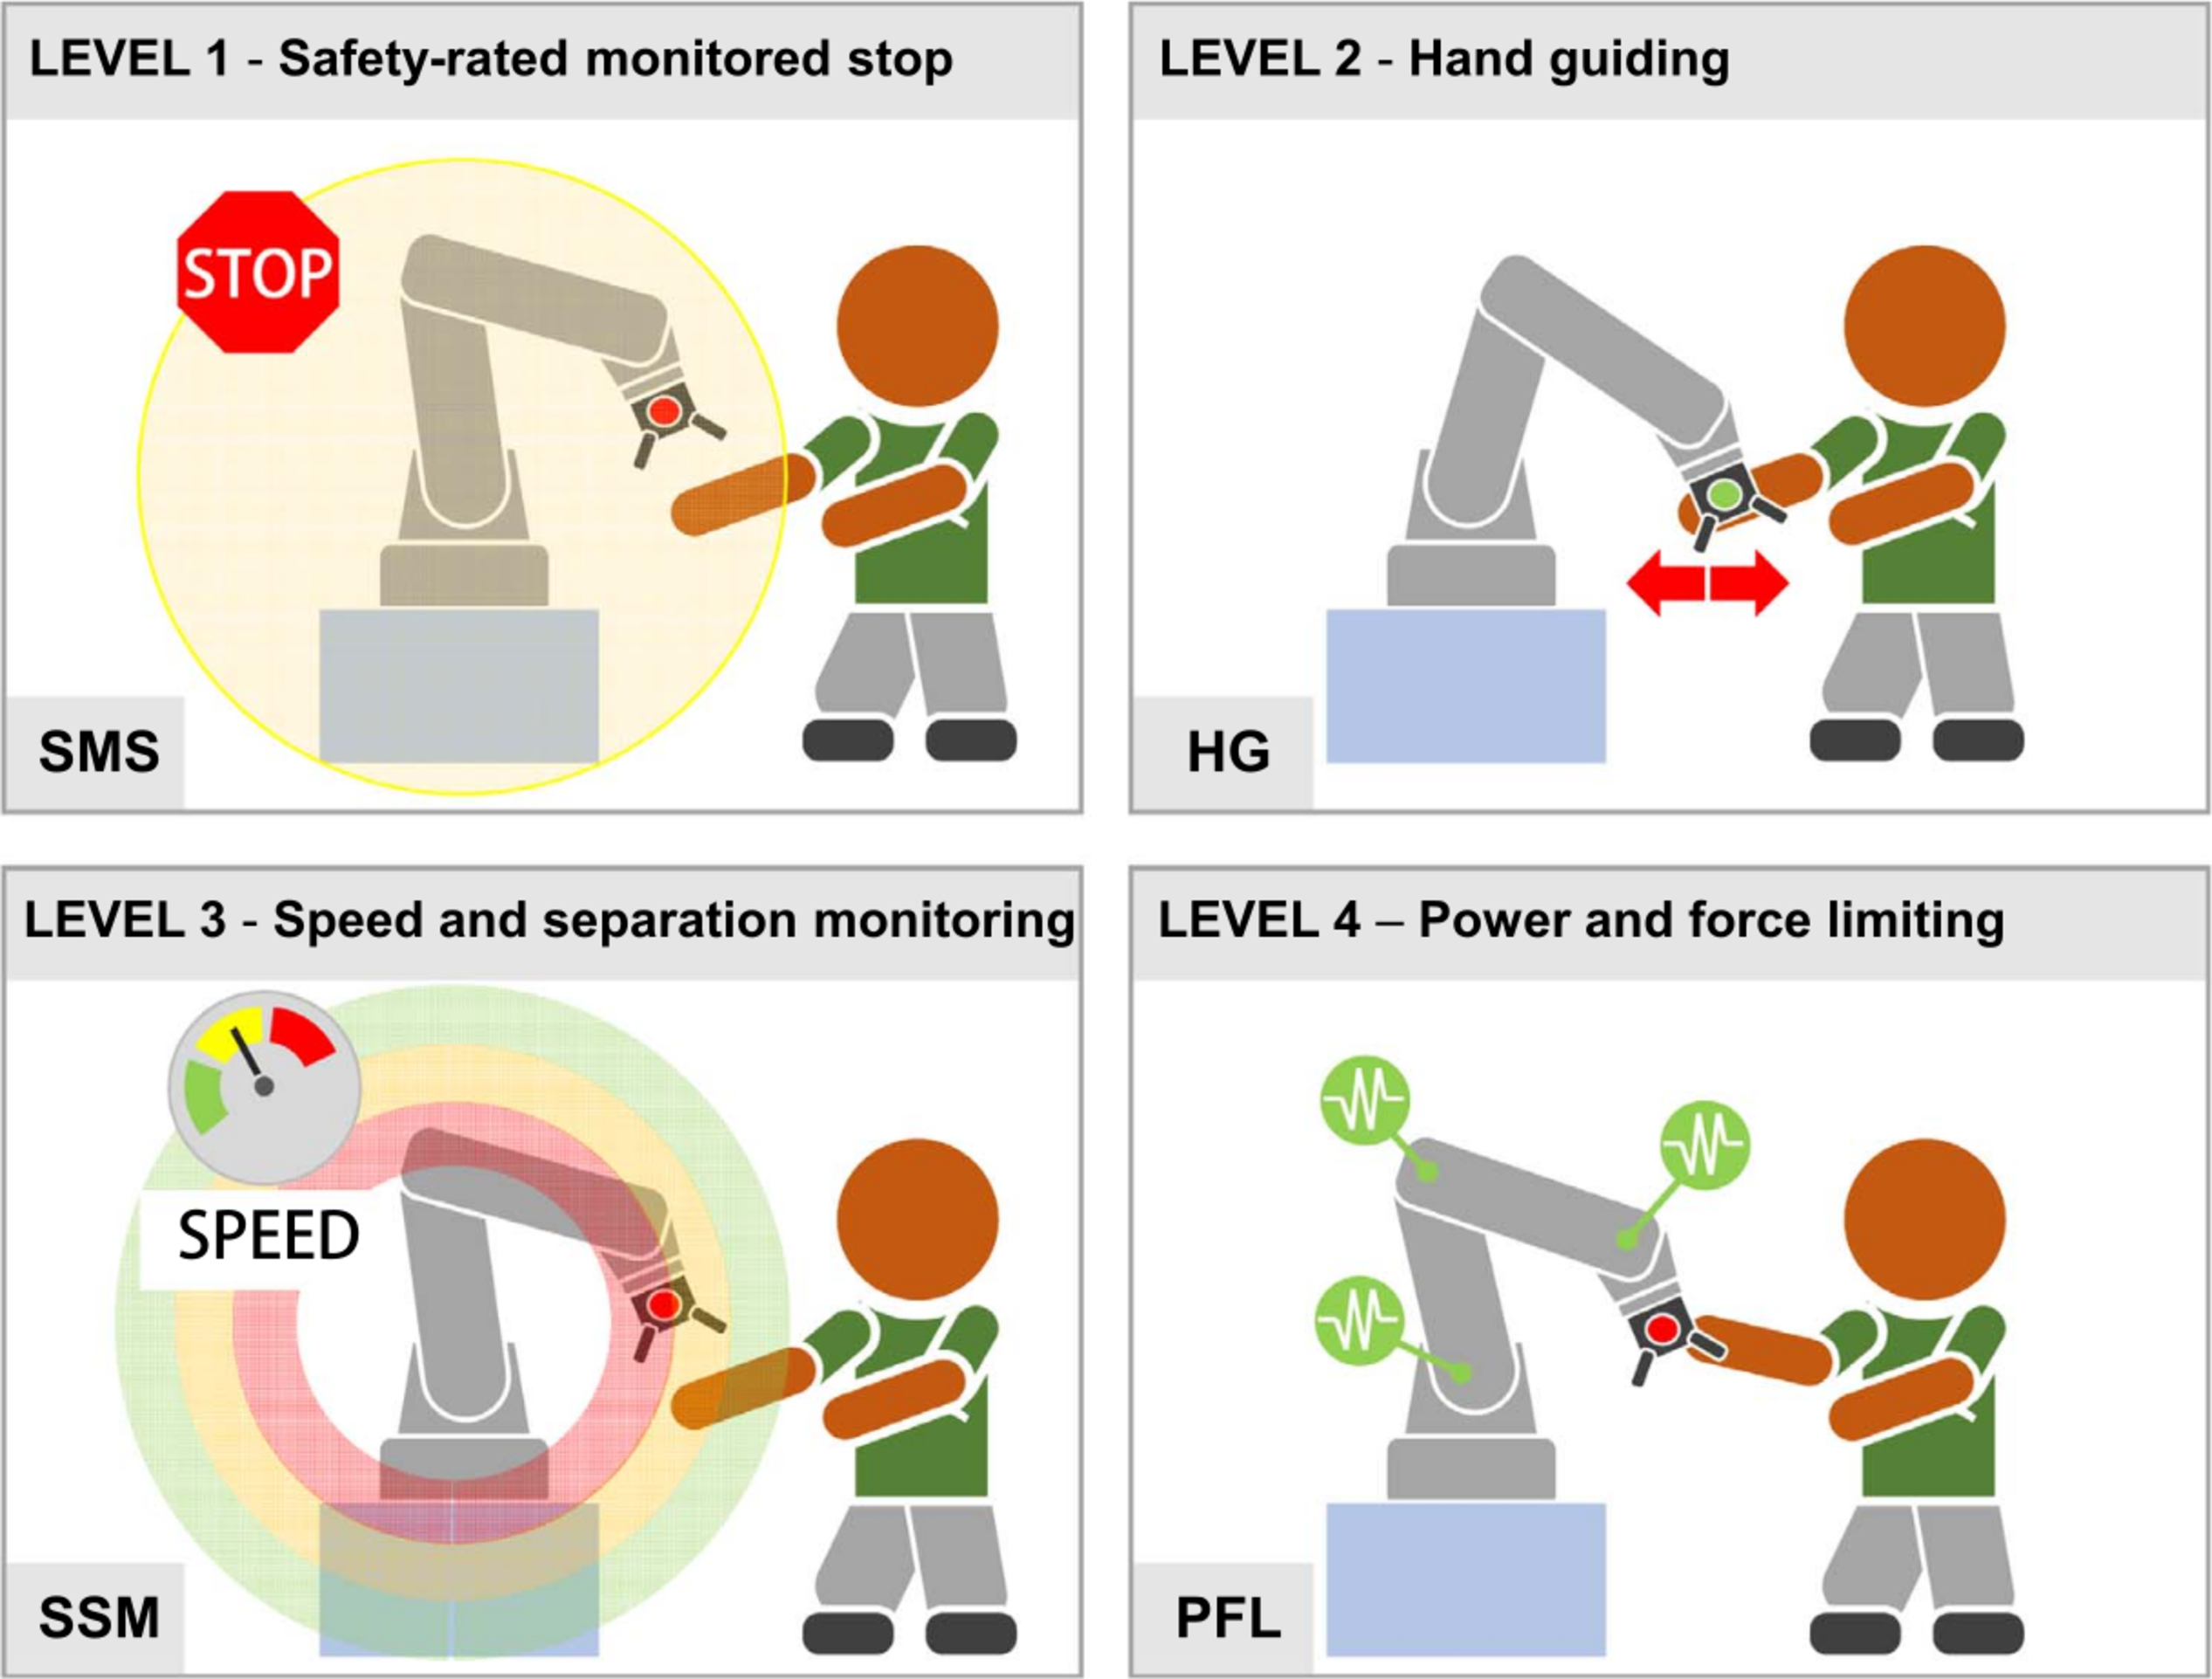
\includegraphics[width=5in]{figs/iso.png}}
\caption[The four collaborative operative modes identified by robot safety standards ISO modes 10218-1/2]{The four collaborative operative modes identified by robot safety standards ISO modes 10218-1/2 \cite{Villani2018}}
\label{isonorms}
\end{figure}

\section{Data Sources and Sensors}

The first step to anticipating the following action is to know which sensors should be used. Previously, several forms of communication between humans and robots were described. Still, these work in a more active way, and not all of them can be applied to action anticipation, where the user should not need to do anything for the robot to act. Essentially, there is a need to capture the human's body language or, in other words, his involuntary pose, gestures and gaze, which became some of the most commonly used data to perform action anticipation.

Regarding the sensors used to capture the raw data, most literature suggests using an RGB camera. However, the captured images may be used in the following different ways:

\begin{itemize}
\item directly used as input to models which can extract features from the images;

\item used as input to frameworks that receive an image, process it, and return the key points, such as the skeleton joints of the person in the image; these key points can also then be used to assume the gaze of the human in the image such as in \textcite{Canuto2021} where the authors used OpenPose (explored in detail in Section \ref{section:keypointdetection}) to obtain not only the skeleton joints but also the worker's gaze;

\item used to process the optical flow\cite{Gammulle2019, Wu2021, Rodriguez2019, Furnari2021};

\item if the human was wearing markers, the image can be used to obtain the positions of the markers obtaining gestures from the sequence of those positions \cite{Maeda2016};
\end{itemize}

Besides RBG cameras, some works, such as the one described in \textcite{Moutinho2023}, indicate the use of an RGB-D camera to capture both the color and the depth images, which contain the gestures and pose of the worker. Other than cameras, in \textcite{Tortora2019} \acs{imu} and \acs{emg} data was used as input to capture the gestures and anticipate the worker's action. When it comes to obtaining the worker's gaze, it is possible to do so from the RGB images as mentioned above, but it is also possible to use wearable sensors to capture it, such as in \textcite{Schydlo2018}.

\section{Methods}

% 1 modelo
% 2+ modelo
% modelo+decision making
% modelo+decision making+motion planning

After knowing which data is usually captured and provided to an algorithm, this section explores possible algorithmic solutions present in previous work starting by those that are only about predicting the action of the human worker and then those that go a step further and reference how to go from a prediction to the action that the robot must execute as a response.

\subsubsection{Predictive Modeling Techniques}

Predicting the next action of the worker can be represented as a classification problem since it is possible to use a sequence of images that must be classified as a particular future action class. Using Fig.~\ref{superviseddiagram} as an example, the high-five action should be predicted before the frames that contain it are captured. The previous work with this kind of algorithm mainly includes \acp{cnn} and \acp{rnn}, with the latter being the most common.

\begin{figure}[H]
\centerline{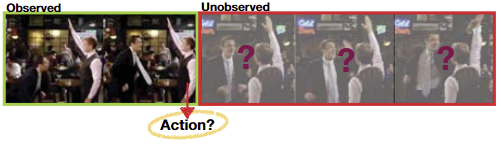
\includegraphics[width=6in]{figs/superviseddiagram.PNG}}
\caption[Action Anticipation using Supervised Learning diagram]{Action Anticipation using Supervised Learning diagram\cite{Gammulle2019}}
\label{superviseddiagram}
\end{figure}

% LSTM only examples
In \textcite{Furnari2021}, the authors aimed to predict the subsequent actions that someone wearing a camera would perform and the objects he would interact with. They used three datasets containing RBG frames from which they derived the optical flow and the objects in the environment. This data is then passed on to a Rolling-Unrolling \acs{lstm}. The Rolling \acs{lstm} (R-\acs{lstm}) is a network that continuously encodes the received observations and keeps an updated summary of the past. When it is time to make predictions about future actions, the Unrolling \acs{lstm} (U-\acs{lstm}) is used with its hidden and cell states equal to the current ones of the R-\acs{lstm}.

In \textcite{Schydlo2018}, the authors used an encoder-decoder recurrent neural network topology to predict human actions and intent where the encoder and the decoder are both \acs{lstm} cells. At each step, the decoder returns a discrete distribution of the possible actions making this algorithm able to consider multiple action sequences, which are then subject to a pruning method that reduces them to obtain the right action finally. In their work, these algorithms were tested in two different datasets, one containing RGB images with optical markers and gaze information from wearable sensors and another with RGB-D images.

% ResNet-34 + LSTM
In \textcite{Moutinho2023}, the authors aimed to increase the natural collaboration between the robot and the human in an assembly station by interpreting implicit communication cues. The data related to the environment was captured using an RGB-D camera. This data was then passed on to a ResNet-34, a pre-trained neural network that extracted the features from the images. These features are used as the input to a \acs{lstm} to perform human action recognition.

% ResNet-50 + LSTM
In \textcite{Gammulle2019}, the authors aimed to predict future frames while at the same time predicting the following action. In their implementation, they used public datasets with videos from which they obtained RGB images and optical flow streams. To consider both data sources, they also used two ResNet-50's, which are pre-trained networks, one to get the input features from the image and another from the optical flow, and 2 \acp{lstm} to take into account both sequences of inputs. Then the two results are merged into a final classification. They also used two Generative Adversarial Networks (GAN) to generate the subsequent frames, but this is different from the focus of the analysis.

%% VGG-16 + TTM
In \textcite{Wang2021}, the authors used video datasets to train a model that would predict a future action from the observed frames. They used three pre-trained neural networks in their work: VGG-16, TS, and ConvNet, to extract features from the images. Then these features were aggregated using a Temporal Transformer module (TTM), and finally, a progressive prediction module (PPM) would anticipate the worker's future action. This article also addresses the issue of specifying what the algorithm should consider as an action. Although most of the literature often implies that the last frames captured by the camera are considered an action, given that those are the frames that contain the last action made by the user, the authors of this article go into greater detail. They tested and evaluated how many frames should be considered as the last action to obtain the best results using a metric from \textcite{Geest2016} named per-frame calibrated average precision (cAP) calculated with \eqref{eq}. In \cite{Wang2021} it is defined with
\begin{equation}
cAP=\frac{\sum_k cPrec(k) * I(k)}{P},
\label{eq}
\end{equation}
\textquote{... where  calibrated  precision $cPrec=\frac{TP}{TP+FP/w}$, $I(k)$ is an indicator function that is equal to 1 if the cut-off frame k is a true positive, $P$ denotes the total number of true positives, and $w$ is the ratio between negative and positive frames. The mean cAP over all classes is reported for final performance.}.

%% CNN
In \textcite{Rodriguez2019}, the authors aimed to predict the following action by first predicting the following motion images. They used datasets containing videos and then processed them to obtain motion images. These motion images become the input of a convolutional autoencoder network that generates the following motion images. These images are then passed to a \acs{cnn} that processes them and makes action predictions for the future. The final action prediction is obtained from the results of the previous network and those of a second \acs{cnn}, which analyzes the original RGB images.

%% architecture with TSN
In \textcite{Wu2021}, the author's goal was to predict the following action someone wearing a camera would perform after some time. Initially, the optical flow was obtained from the captured images, and both were used as input to the model. The model is comprised of a Temporal Segment Networks (TSN), a \acs{cnn}, and a \acs{lstm} to predict the future frame features and then use them to perform the required classification.

\subsubsection{From Prediction to Planning}

After predicting the next action of the worker, the robot must execute some action as a response to complete the anticipation process. This subsubsection contains articles that go beyond the predictive model and have relevant details for the integration of the model in a controller.

In \textcite{Canuto2021}, the authors aimed to predict the following action using a \acs{lstm}, one of the most common \acp{rnn}. In their work, they used a dataset captured with an RGB camera. From these images, they obtained the objects in the environment, the human skeleton joints extracted over time using OpenPose, and the gaze derived from the joints. Then the three data sources were given to the \acs{lstm} as input to perform the desired classification. In this process, the authors use an adaptive threshold on the uncertainty of the recurrent neural network, which makes the model need a certain level of certainty to classify the action as a particular class. This creates a more robust solution since a standard supervised learning algorithm would predict the class with the highest probability even if the model has low certainty about every category.

% Look-up table
In \textcite{Maeda2016}, the authors aimed to reduce the delay in the robot's response by anticipating the human worker and providing a screw or a plate accordingly. They captured the environment using an RGB camera and tracked the hand using optical markers. Then they predicted the following human action using a look-up table containing different orders for assembly actions. With the nearest neighbor algorithm, the actions of the human would be matched with a particular order. The limitation of this method is that all possible sequences need to be on the table because if they are not there, then the robot will match with a different order which may be undesirable. If the robot eventually notices that it did the wrong action, it would then follow a hard-coded contingency trajectory to return to the pre-grasping position. When performing a handover action, the previously captured data is used to generate possible trajectories and this is given to the feedback controller as a reference.

% LSTM + CNN
In \textcite{Zhang2022}, the authors aimed to predict the intention of the human worker to provide him with the required piece. To achieve this, they used an RGB camera to capture the data from the environment. Then the images are given to a convLSTM framework where the \acs{cnn} part is in charge of extracting features from the input images, and these features are then passed on to the \acs{lstm} to predict the intention. This article also tackles the issue of having several possible assembly orders. It solves it by creating a phase at the beginning of the collaboration in which the robot learns the assembly actions and their order from a demonstration. After the prediction of the intention of the worker, the robot proceeds to fetch the required piece. It uses a \acs{cnn} to recognize said piece and \acs{ros} Open Motion Planning Library (OMPL) to handle the trajectory planning jobs. In terms of safety, the authors defined speed limits for the robot and ensured that the robot would avoid the workspace of the human. Then when it needs to move closer to the user, its speed is reduced to guarantee the user's safety.

In \textcite{Huang2016}, the authors' goal is to make the robot use the anticipated actions of the worker to decide its tasks. It monitors the worker's gaze using a wearable device and uses it to predict his intent using SVM. After predicting it, the robot uses an anticipatory motion planner named \textquote{MoveIt!} to plan its motion according to a certain confidence threshold. This means that while it is unsure of what the human wants, the robot starts to move towards the item it thinks he wants but only really moves completely when it surpasses the threshold.

\if{0}
% POMDP
In \textcite{Gorur2018}, the authors aimed to make the human-robot interaction more natural by detecting unexpected conditions where the human will not need the robot's assistance, such as when the human's current intention is unknown or irrelevant to the robot or when even though the human's intent is relevant, that task is done only by the human. They used the algorithm Partially Observable Markov Decision Process (POMDP) to achieve this. The training was done with simulation with the model learning a policy by having a positive reward if the task was accomplished and a negative reward if the robot tried to help the human in a situation where it should not.

\section{\textcolor{red}{\acl{hrc} Safety}}

\textcolor{red}{potentially join this content with the previous subsubsection}

Finally, safety is a topic that must always be mentioned when robots work with humans, especially in \acs{hrc}. Although this topic was also covered in subsection \ref{subsection:collaborative_robotics}, many articles in action anticipation also explore their strategies to ensure the worker's safety.

In \cite{Psarakis2022}, the authors attempted to create a sense of anticipation in humans towards the robot's movements through visual cues of the robot's upcoming action, which is the reverse of what it is being tried to achieve in the other reviewed papers. As with the previous article, they also made it so the robot must reduce its movement speed when close to the robot. Although it was only tested in the Virtual Reality simulation shown in Fig.~\ref{vr}, where the users feel safer, they concluded that the efficiency of the collaboration was increased, and the user had a greater feeling of safety and trust. Furthermore, knowing what the robot will do next also decreases the risk of a collision since the user will avoid the space where the robot is working, increasing safety.

\begin{figure}[H]
\centerline{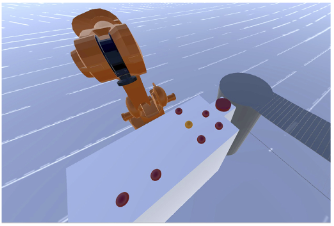
\includegraphics[width=3.5in]{figs/reverse.PNG}}
\caption{VR Simulation of \cite{Psarakis2022}, the orange means the robot will pick that puck next}
\label{vr}
\end{figure}

In \cite{Mukherjee2022}, it is also stated that limiting the power and force of the robot decreases the gravity of the consequences of a possible collision, increasing safety.
\fi
\chapter{Materials and Methods}
\label{chapter:materials_and_methods}

This chapter covers a review of the experimental infrastructure including relevant hardware and software tools used while developing the final solution.

\section{Hardware Setup}

The experimental part of this thesis was developed using the setup available at the Laboratory for Automation and Robotics (LAR) located in the Department of Mechanical Engineering at the University of Aveiro. This setup was designed to meet the requirements of the AUGMANITY mobilizing project\footnote{AUGMANITY website: \url{https://www.augmanity.pt}} and it contains an UR10e collaborative robot and multiple cameras, including the Orbbec Astra Pro RGBD camera which was utilized.

\textcolor{red}{Image of the setup}

\subsection{UR10e Robot}

UR10e is a collaborative robot model developed by Universal Robots focused on versatility. It allows for payloads up to 12.5 kg and has a reach of 1300mm being suitable for tasks such as machine tending, palletizing, and packaging\cite{UR10e}. The one used in this work is equipped with a \textcolor{red}{(missing gripper model)} gripper.

\begin{figure}[h]
\centerline{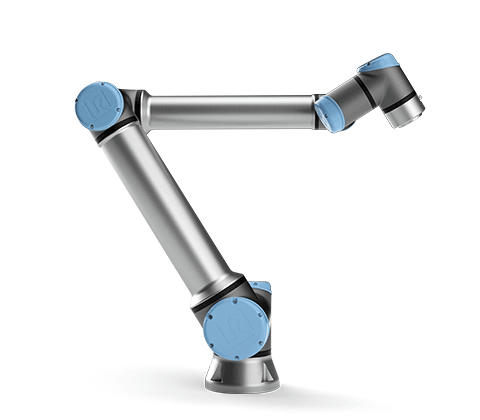
\includegraphics[height=2.5in]{figs/UR10e.png}}
\caption[UR10e]{UR10e collaborative robot \cite{UR10e_image} \textcolor{red}{(missing gripper image)}}
\label{fig:ur10e}
\end{figure}

\subsection{Orbbec Astra Pro}

Orbbec Astra Pro is an RGBD camera developed by Orbbec Technologies. It is frequently used in computer vision and robotics for tasks such as face recognition, gesture recognition, human body tracking, three-dimensional measurement, environment perception, and three-dimensional map reconstruction\cite{AstraPro}. In this work, the camera is placed above the environment facing down capturing both color and depth real-time images.

\begin{figure}[h]
\centerline{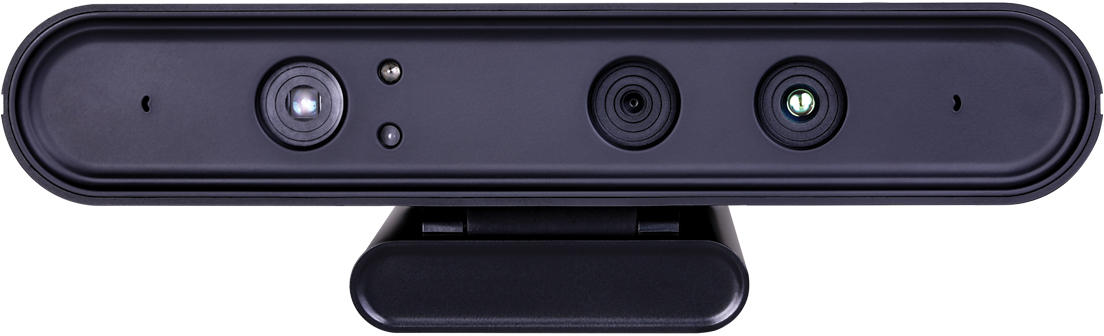
\includegraphics[height=1.2in]{figs/Astra.jpg}}
\caption[Orbbec Astra Pro]{Orbbec Astra Pro \cite{AstraPro}}
\label{fig:orbbec_astra_pro}
\end{figure}

\section{Software Tools}

\subsection{\acf{ros}}

\acs{ros}\cite{ROS2}\footnote{\acs{ros} 1 documentation: \url{https://wiki.ros.org}}\footnote{\acs{ros} 2 documentation: \url{https://docs.ros.org/en/humble}} is an open-source collection of tools and software libraries used to develop a robotics application. Its main features are:

\begin{itemize}
    \item \textbf{message broker}: every process in the project is a node in the \acs{ros} network and communicates with the other nodes mainly through topics (asynchronous publish/subscribe streaming of data) or services (synchronous RPC-style communication);
    \item \textbf{code reuse}: executables and packages are written to be as independent as possible, making the developer able to reuse them in another project;
    \item \textbf{rich ecosystem}: there are several open-source packages available to the developer that can be easily integrated;
    \item \textbf{scalability}: given that the nodes are so loosely coupled, it allows for node distribution;
    \item \textbf{language independence}: nodes can be written in any language since communication is established through well-defined objects;
    \item \textbf{data visualization}: there are tools to visualize the data in real-time, such as Rviz;
    \item \textbf{simulator support}: \acs{ros} has support for simulators with Gazebo being the most common;
    \item \textbf{hardware abstraction}: contains driver packages to deal with some hardware devices;
\end{itemize}

In this work, \acs{ros} is used to establish communication throughout all of the infrastructure. This makes it easier to integrate with previously developed software for the robot and set up the necessary drivers both for the robot and the camera. Additionally, Rviz is used to help visualize the functioning of the system.

\subsection{MoveIt}

MoveIt\footnote{MoveIt documentation: \url{https://ros-planning.github.io/moveit_tutorials}} is a widely-used open-source framework for robotics applications involving motion planning, manipulation, 3D perception, kinematics, control, navigation, and collision checking. MoveIt is implemented on top of ROS taking advantage of the latter's features such as the messaging and build systems as well as standard tools such as ROS Visualizer (Rviz) and the ROS robot format (URDF).

In this work, the MoveIt framework is used to plan and execute the robot arm movements with OMPL, an open-source motion planning library used by MoveIt for motion planning tasks.

\subsection{Tensorflow}

Tensorflow\footnote{Tensorflow documentation: \url{https://www.tensorflow.org/api_docs}} is a platform that can be used for all steps of a machine learning project. Its main features are:
\begin{itemize}
    \item \textbf{prepare data}: load data, data pre-processing and data augmentation;
    \item \textbf{build models}: design and train custom models with little code or use pre-trained ones (transfer learning);
    \item \textbf{deploy models}: helps using models in different platforms such as locally, in the cloud, in a browser, or in mobile;
    \item \textbf{implement MLOps}: run models in production, tracking their performance and identifying issues.
\end{itemize}

In this work, Tensorflow is used to design and train the machine learning models.

\section{Methods}

This section explains the methods used in this work in greater detail.

\subsection{LSTM}

\subsection{Transformer Neural Networks}

Transformer Neural Networks consist of a new kind of neural network architecture that aims to solve tasks involving sequence data such as those in natural language processing. They were initially proposed in the "Attention Is All You Need" paper published by Google Research in 2017\cite{Vaswani2017} and proceeded to surpass several established architectures in numerous tasks using attention mechanisms that identify complex relationships between elements in the input sequence.

According to \textcolor{red}{https://learning.oreilly.com/library/view/deep-learning-with/9781803232911/}, the transformer's architectures are built upon 4 core concepts: positional encoding, attention, self-attention, and multi-head (self-)attention.

\subsubsection{Positional encoding}

RNNs are able to work with sequences given that the tokens are processed sequentially. However, this approach comes with the disadvantage of the model having greater difficulty in analyzing long sequences, since important data might be forgotten. Transformers address this issue by using positional encoding, assigning a unique number to each token representing its position in the input sequence. This enables the transformer to learn the significance of each token's position.

\subsubsection{Attention}

Attention is a concept that consists in measuring the relative importance of the input tokens to the output tokens. It was initially designed to facilitate language translation given that, when translating text from one language to the other, each word in the output can be influenced by multiple words from the input, and it became a key idea behind the transformer's architecture.

\subsubsection{Self-attention}

Self-attention derives from attention but consists in measuring the relative importance of the input tokens to the other tokens of the input sequence instead of the output tokens. This concept allows the model to learn the relationships between tokens and their relevance in the input sequence even if they are far away.
 
\subsubsection{Multi-head (self-)attention}

Multi-head (self-)attention refers to the fact that a transformer can have multiple attention heads. Each attention head performs a parallel process of (self-)attention allowing for multiple resulting weight matrices and, therefore, multiple definitions of relevance between the tokens.

\subsubsection{Architecture}

\begin{figure}[h]
\centerline{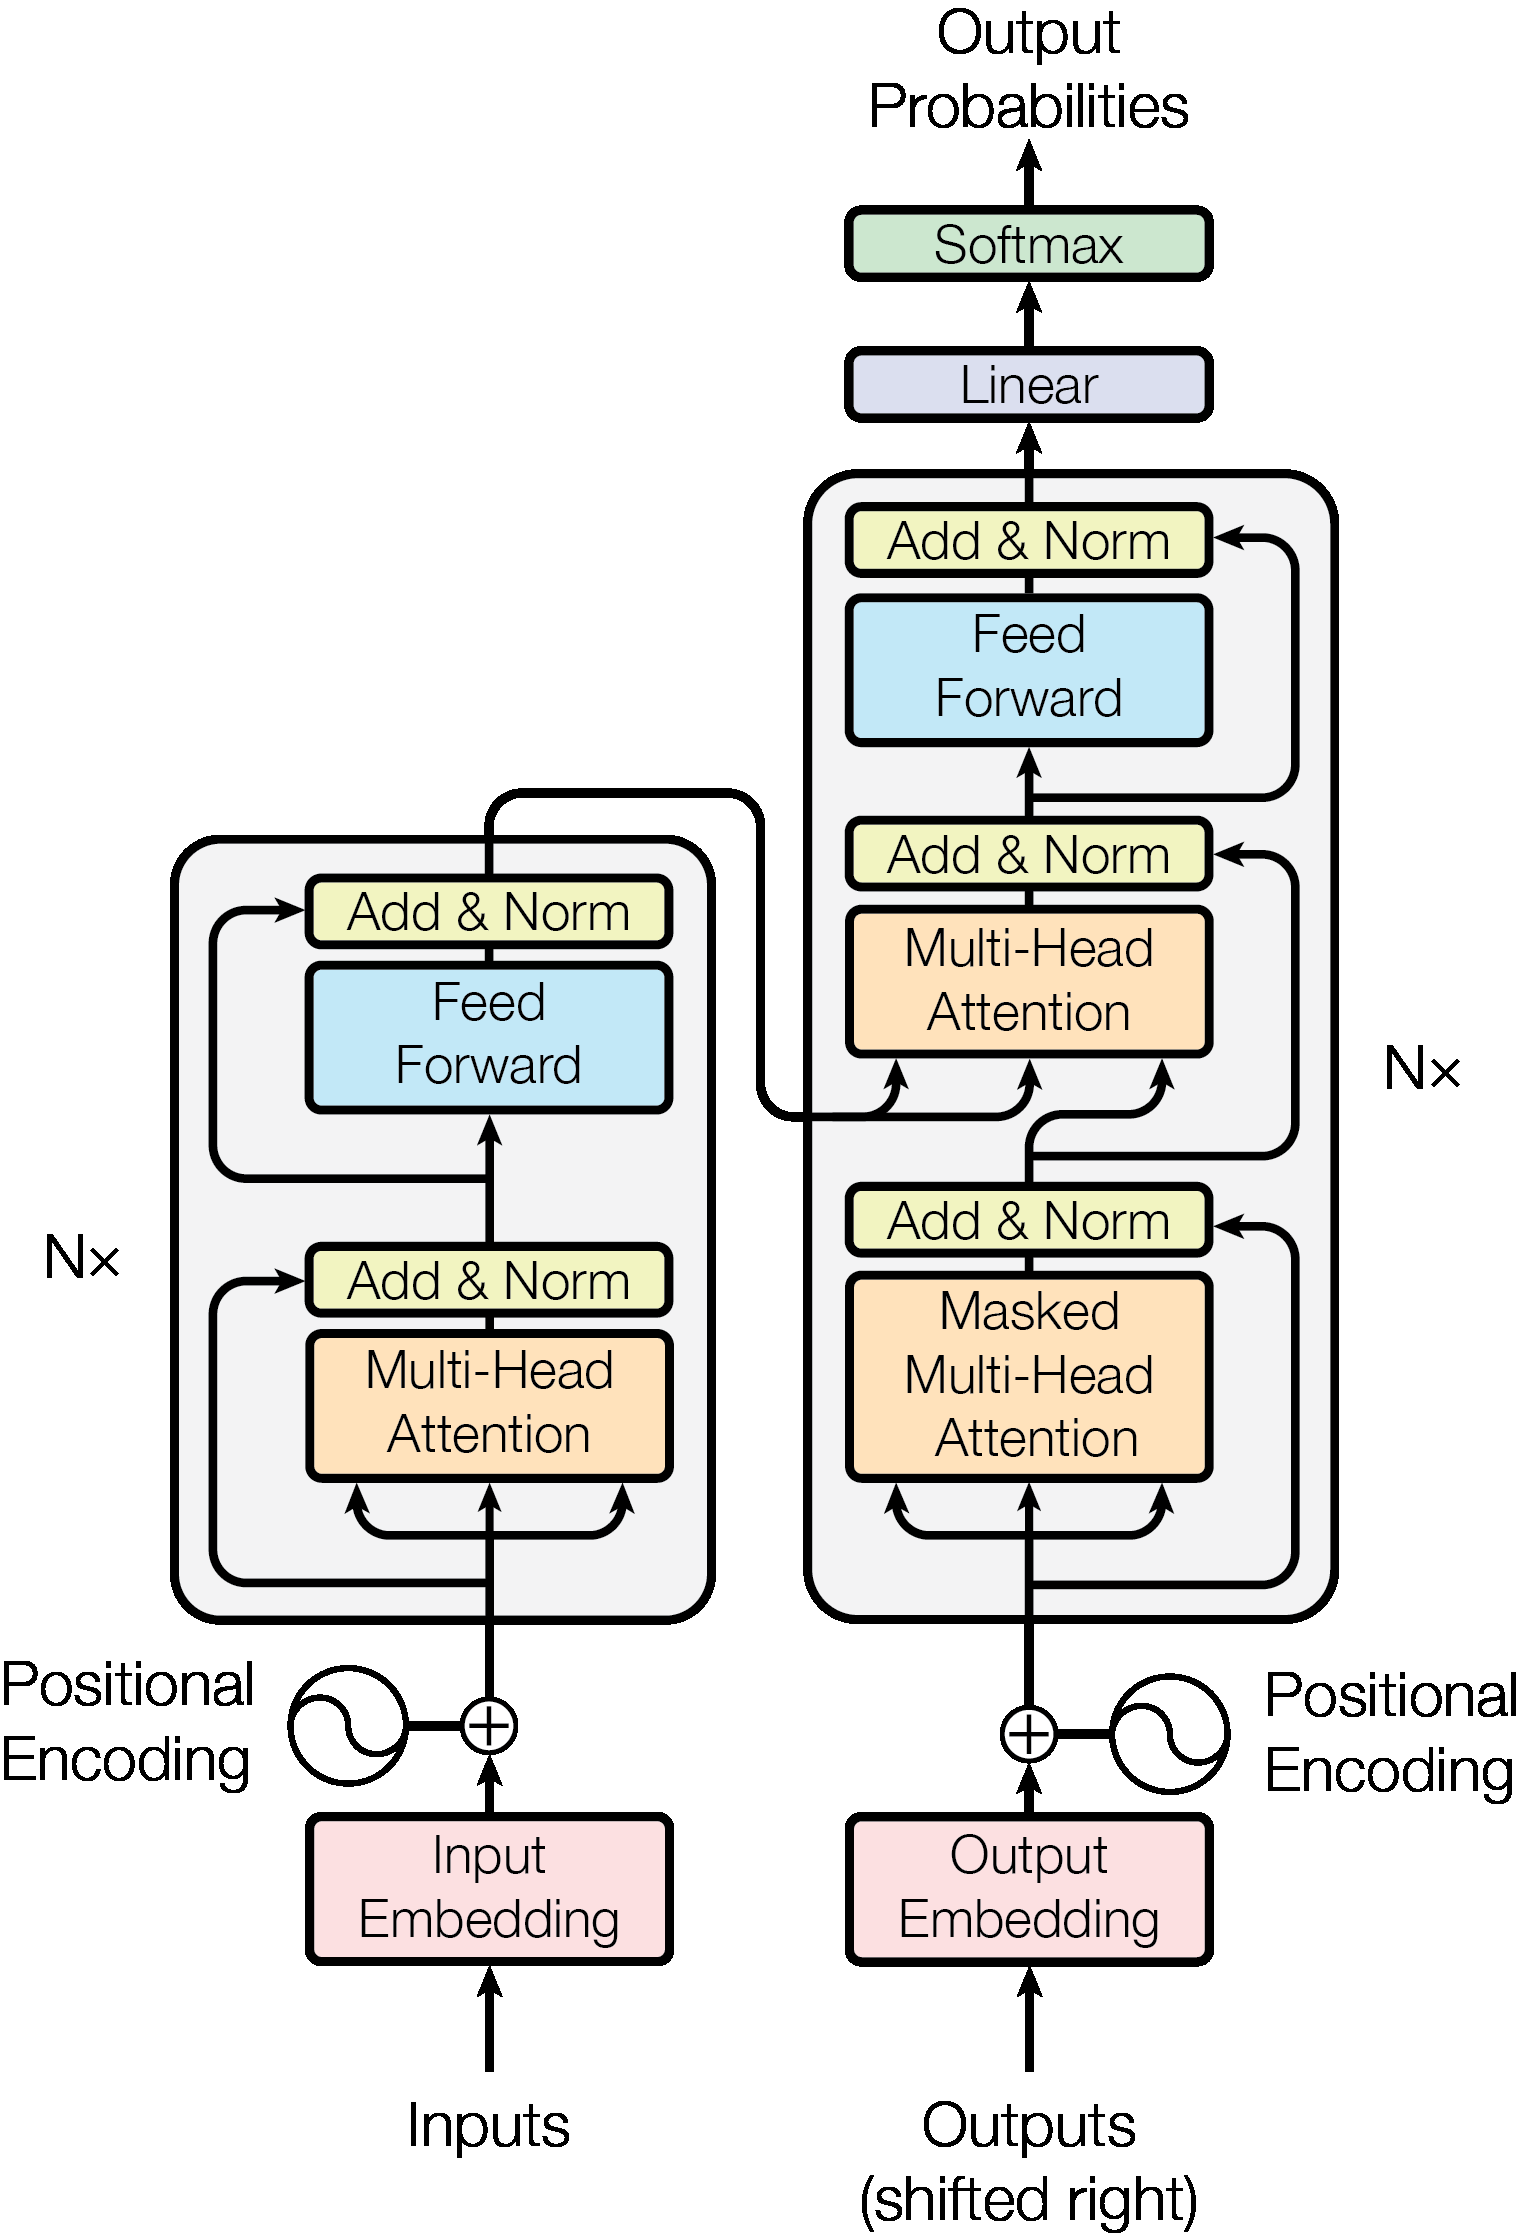
\includegraphics[height=6in]{figs/transformer.jpg}}
\caption[Transformer Architecture]{Transformer Architecture \cite{Vaswani2017}}
\label{fig:transformer_arch}
\end{figure}

\chapter{Robot Controller}
\label{chapter:robot_controller}

This chapter covers the implementation of the robot controller including the workflow of the different solutions, the general ROS architecture, and the details of the state machine.

\if{0}

{\color{red} \rule{\linewidth}{0.5mm}}

{\color{gray}
\section{First Work (possibly to remove)}

The first version developed comprised simple actions that were triggered by sensor data based on a set of rules with the end goal of building a tower of blocks with 3 possible orders. Additionally, the system was able to recover from mistakes.

\textcolor{red}{maybe an image with the different orders to better visualize the solution?}

\subsubsection{State Machine Logic}

This version was developed as a state machine with 7 different states, as shown in Fig.~\ref{fig:demo1_state_machine}.

\begin{figure}[H]%[!ht]
    \centering
    \begin{tikzpicture}[
        > = stealth, % arrow head style
        shorten > = 1pt, % don't touch arrow head to node
        auto,
        node distance = 3.5cm, % distance between nodes
        semithick % line style
    ]
    
    \tikzstyle{every state}=[
        draw = black,
        thick,
        fill = white,
        minimum size = 4mm,
        text width = 1.5cm,
        align = center
    ]
    
    \node[state] (idle) at (0,0) {idle};
    \node[state] (picking_up) [right of=idle] {picking up};
    \node[state] (waiting) [right of=picking_up] {waiting};
    \node[state] (moving_closer) [right of=waiting] {moving closer};
    \node[state] (putting_down) [below of=picking_up] {putting down};
    \node[state] (stop_side_switch) [below right of=moving_closer] {stop side switch};
    \node[state] (stop_wrong_guess) [above of=picking_up] {stop wrong guess};
    
    % \path[->] (idle) edge node[align=center] {received new\\sequence} (picking_up);
    % \path[->] (picking_up) edge node[align=center] {object\\picked up} (waiting);
    % \path[->] (waiting) edge node[align=center] {user\\finished} (moving_closer);
    % \path[->] (moving_closer) edge node[align=center] {robot in put\\down position} (putting_down);
    % \path[->] (putting_down) edge node[align=center] {object\\put down} (picking_up);
    % \path[->] (putting_down) edge[bend left] node[align=center] {sequence\\finished} (idle);
    % \path[->] (moving_closer) edge[bend left] node[align=center] {user changed\\side} (stop_side_switch);
    % \path[->] (stop_side_switch) edge[bend left] node[align=center] {robot\\stopped} (moving_closer);
    % \path[->] (picking_up) edge[bend right] node[align=center] {} (stop_wrong_guess);
    % \path[->] (waiting) edge node[align=center] {} (stop_wrong_guess);
    % \path[->] (moving_closer) edge[bend right] node[align=center] {wrong assembly\\sequence} (stop_wrong_guess);
    % \path[->] (stop_wrong_guess) edge[bend right] node[align=center] {reverted\\previous guess} (picking_up);

%Alternative lay-out for easier global configuration (vsantos)
\path[every edge,
	->,
	text width=1.5cm,
	align=center,
    every node/.style={
	   font={\small\sffamily},
        },
%	pos=0.4,
	]
(idle)             edge             node {received new sequence}   (picking_up)
(picking_up)       edge             node {object picked up}        (waiting)
(waiting)          edge             node {user finished}           (moving_closer)
(moving_closer)    edge[pos=0.7]    node {robot in put down position} (putting_down)
(putting_down)     edge             node {object put down}         (picking_up)
(putting_down)     edge[bend left]  node {sequence finished}       (idle)
(moving_closer)    edge[bend left]  node {user changed side}       (stop_side_switch)
(stop_side_switch) edge[bend left]  node {robot stopped}           (moving_closer)
(picking_up)       edge[bend right] node {}                         (stop_wrong_guess)
(waiting)          edge             node {}                         (stop_wrong_guess)
(moving_closer)    edge[bend right] node {wrong assembly sequence} (stop_wrong_guess)
(stop_wrong_guess) edge[bend right] node {reverted previous guess} (picking_up)
; 
    
\end{tikzpicture}
    \caption{First Version - State Machine}
    \label{fig:demo1_state_machine}
\end{figure}

\begin{itemize}
    \item \textbf{idle}: State corresponding to when the robot does not know which is the next assembly sequence. When it receives a new sequence because the user chose the first block then the state changes to $picking$ $up$.
    \item \textbf{picking up}: State corresponding to while the robot is picking up a certain block. After it picks it up the state changes to $waiting$ unless it was picking the wrong object in which case it changes to $stop$ $wrong$ $guess$.
    \item \textbf{waiting}: State corresponding to the time while the robot is waiting for the user to finish working the previous block. When he finishes that task which is indicated by a block reappearing in the workspace, the state changes to $moving$ $closer$ unless the robot is holding the wrong object in which case it changes to $stop$ $wrong$ $guess$.
    \item \textbf{moving closer}: State corresponding to the movement between the waiting and the put-down position opposite to the user so that the robot does not constrain him. After the robot reaches the put-down position the state changes to $putting$ $down$. If the robot is holding the wrong object then the state changes to $stop$ $wrong$ $guess$ instead and if the user changes side the state changes to $stop$ $side$ $switch$.
    \item \textbf{putting down}: State corresponding to the movement necessary to put down the block in the table and the retreat of the robot outside the user's workspace. If there are still more blocks to give then the state changes to $picking$ $up$ and if there are not then the sequence is finished and the state changes to $idle$.
    \item \textbf{stop side switch}: State corresponding to the action of stopping the robot because the user changed sides. After the robot is stopped the state changes back to $moving$ $closer$.
    \item \textbf{stop wrong guess}: State corresponding to the action of stopping the robot because the first block was rotated indicating a different sequence. If the robot was already holding a block then that block is put back where it was while in this state. After the robot is stopped and it is not holding a block the state changes to $picking$ $up$.
\end{itemize}

\subsubsection{Workflow}
Initially, the robot would wait until it detected a red or green object using color segmentation. This information would help him determine not only the first block but possibly the entire sequence since if started with a red block there would only be one option. If it started with a green block then the orientation of the block would give the system information about which sequence should be used.

Before the robot gives a block to the user, it waits for the user to stop taking care of the previous one. This is implemented by tracking when one block reappears in the color image indicating that the user has stopped working on it.

So that the robot avoids being too close to the user, the position of the user is detected using the depth images and the robots puts down a block in the opposite side of the table. Furthermore, if the user switches to the other side the robot will also switch the put down location.

This solution intrinsically consisted of a set of rules where the movements resulted from the direct communication between the robot and the human. Therefore, it was not yet considered an anticipatory system.
}
{\color{red} \rule{\linewidth}{0.5mm}}

\fi

\section{Controller Solutions Workflow}

This subsection covers the workflow of the different solutions implemented.

\subsection{First Solution - Interaction Based}

The first version developed relied on interactions between the robot and the user. When the user puts his hand above a small block, if the state of the robot is $idle$ then it proceeds to fetch a block of the same color. Additionally, when the user hovers his hand over the violet block while the state of the robot is $picking$ $up$ or $moving$ $closer$, it means that the robot fetched the wrong block so it must stop and put the block back where it was before if it was already picked up.

The interactions in this solution are also the fallback behavior if the methods in the following solutions fail to anticipate the block that the user desires.

\subsection{Second Solution - Probability Based}

The second version implemented consisted in having a database of probabilities that the robot would check to anticipate the block that the user would need next. These probabilities were established according to the possible country flags \textcolor{red}{(missing example)}. However, the first block is still requested by the user and, if the robot exhausts all possibilities that it knows of, the user is able to request the following block using the interactions described in the first solution.

\subsection{Third Solution - Rule Based}

\textcolor{red}{still need to explain this one}

\section{System ROS Architecture}

The communication between the robot, the sensors, and the programming logic is established using Robot Operating System (ROS) with the following 5 main nodes.

\textcolor{red}{a diagram might be a good idea to better visualize the solution}

\subsubsection{orbbec\_camera}

This node is responsible for receiving the color and depth images from the Orbbec camera and publishing them on ROS. In order to control to have better control over the lightness in the environment, the back-light compensation was raised to the maximum.

\subsubsection{human\_locator}

This node is responsible for analyzing the depth images and returning the position of the highest point in a certain region of interest which is then considered as the position of the human in the workspace.

\subsubsection{object\_color\_segmenter}

This node is responsible for analyzing the color images and returning the position of the objects in the workspace using color segmentation.

\subsubsection{decision\_making\_block}

This node is responsible for receiving the information resulting from the sensor data and keeping an internal state machine to decide what actions should be taken and when they should be taken.

\subsubsection{move\_it!}

This is a group of nodes responsible for planning the robot's trajectory in each action.

\subsection{State Machine Logic}

As said before, the decision\_making\_block node contains an internal state machine. Although the logic of some states changes depending on the solution, all implementations follow the same general design represented in the state machine diagram shown in Fig.~\ref{fig:state_machine}.

\begin{figure}[H]%[!ht]
    \centering
    \begin{tikzpicture}[
        > = stealth, % arrow head style
        shorten > = 1pt, % don't touch arrow head to node
        auto,
        node distance = 3.8cm, % distance between nodes
        thick % line style
    ]
    
    \tikzstyle{every state}=[
        draw = black,
        thick,
        fill = white,
        minimum size = 4mm,
        text width = 1.5cm,
        align = center
    ]
    
    \node[state] (idle) at (0,0) {idle};
    \node[state] (picking_up) [right of=idle] {picking up};
    \node[state] (moving_closer) [right of=picking_up] {moving closer};
    \node[state] (putting_down) [below of=picking_up] {putting down};
    \node[state] (stop_side_switch) [right of=moving_closer] {stop side switch};
    \node[state] (stop_wrong_guess) [above of=picking_up] {stop wrong guess};
    
    % \path[->] (idle) edge node[align=center] {received new\\sequence} (picking_up);
    % \path[->] (picking_up) edge node[align=center] {object\\picked up} (waiting);
    % \path[->] (waiting) edge node[align=center] {user\\finished} (moving_closer);
    % \path[->] (moving_closer) edge node[align=center] {robot in put\\down position} (putting_down);
    % \path[->] (putting_down) edge node[align=center] {object\\put down} (picking_up);
    % \path[->] (putting_down) edge[bend left] node[align=center] {sequence\\finished} (idle);
    % \path[->] (moving_closer) edge[bend left] node[align=center] {user changed\\side} (stop_side_switch);
    % \path[->] (stop_side_switch) edge[bend left] node[align=center] {robot\\stopped} (moving_closer);
    % \path[->] (picking_up) edge[bend right] node[align=center] {} (stop_wrong_guess);
    % \path[->] (waiting) edge node[align=center] {} (stop_wrong_guess);
    % \path[->] (moving_closer) edge[bend right] node[align=center] {wrong assembly\\sequence} (stop_wrong_guess);
    % \path[->] (stop_wrong_guess) edge[bend right] node[align=center] {reverted\\previous guess} (picking_up);

%Alternative lay-out for easier global configuration (vsantos)
\path[every edge,
	->,
	text width=1.8cm,
	align=center,
%	pos=0.4,
	]
(idle)             edge             node {knows which block is the next}   (picking_up)
(picking_up)       edge             node {object picked up}        (moving_closer)
(moving_closer)    edge[bend left]  node {robot in put down position} (putting_down)
(putting_down)     edge[bend left]  node {robot retreated}         (idle)
(moving_closer)    edge[bend left]  node {user changed side}       (stop_side_switch)
(stop_side_switch) edge[bend left]  node {robot stopped}           (moving_closer)
(picking_up)       edge             node[right] {wrong assembly sequence}                         (stop_wrong_guess)
(moving_closer)    edge[bend right]  node[above right] {wrong assembly sequence} (stop_wrong_guess)
(stop_wrong_guess) edge[bend right]  node[above left] {reverted previous guess} (idle)
; 
    
\end{tikzpicture}
    \caption{State Machine}
    \label{fig:state_machine}
\end{figure}

\begin{itemize}
    \item \textbf{idle}: State corresponding to when the robot does not know which is the next block. If the sequence has not started yet then it waits for the user to choose the first block and then the state changes to $picking$ $up$. If the sequence has already started then the database is fetched for the possible next blocks and then if at least one block is returned the state changes to $picking$ $up$ or if none is returned the system waits for the user to choose the next block.
    \item \textbf{picking up}: State corresponding to while the robot is picking up a certain block. After it picks it up the state changes to $moving$ $closer$ unless it was picking the wrong object in which case it changes to $stop$ $wrong$ $guess$.
    \item \textbf{moving closer}: State corresponding to the movement until the put-down position opposite to the user so that the robot does not constrain him. After the robot reaches the put-down position the state changes to $putting$ $down$. If the robot is holding the wrong object then the state changes to $stop$ $wrong$ $guess$ instead and if the user changes side the state changes to $stop$ $side$ $switch$.
    \item \textbf{putting down}: State corresponding to the movement necessary to put down the block in the table and the retreat of the robot outside the user's workspace. After that, the state changes to $idle$.
    \item \textbf{stop side switch}: State corresponding to the action of stopping the robot because the user changed sides. After the robot is stopped the state changes back to $moving$ $closer$.
    \item \textbf{stop wrong guess}: State corresponding to the action of stopping the robot because the user indicated that it was the wrong block. If the robot was already holding a block then that block is put back where it was while in this state. After the robot is stopped and it is not holding a block the state changes to $picking$ $up$ if there are still more possible blocks in the database. Otherwise, the state changes to $idle$ so that it waits for a user request.
\end{itemize}


\chapter{Learning}
\label{chapter:learning}

This chapter covers the learning part of this dissertation including data collecting, dataset preprocessing, and the models' structures and optimizations.

\section{Problem Introduction}

When anticipating the next action of the user, the object that the user is grasping can provide crucial information about the user's intention. Although an object detection algorithm may be helpful they can suffer from occlusion problems. Therefore, the following models attempt to solve this problem by taking an image of the user grasping a certain object and classifying which object is being grasped using the geometry of the hand.

To obtain a model that would be able to achieve the previous objective two experiments were made. In the first experiment, some types of models were tested with a smaller dataset containing only 300 images per object and 3 objects with the aim of knowing if they would be worth using and optimizing in a more complex problem. In the second experiment, a bigger dataset with 3000 images per object and 4 objects was used to train and optimize the models.

\begin{figure}[H]%[!ht]
    \centering
    \begin{tikzpicture}[>=latex']
    \tikzset{block/.style= {draw, rectangle, align=center,minimum width=3cm,minimum height=1cm},
    rblock/.style={draw, shape=rectangle,rounded corners=1.5em,align=center,minimum width=2cm,minimum height=1cm},
    input/.style={ % requires library shapes.geometric
    draw,
    trapezium,
    trapezium left angle=60,
    trapezium right angle=120,
    minimum width=2cm,
    align=center,
    minimum height=1cm
    },
    }
    
    
    \node [rblock] (camera) {Camera\\Image};
    \node [block, right =3cm of camera] (hands_keypoints) {Mediapipe\\Hands\\Model};
    \node [block, right =3cm of hands_keypoints] (body_keypoints) {Mediapipe\\Full Body\\Model};
    \node [block, below =2cm of body_keypoints] (normalization) {Points\\Normalization};
    \node [block, left =3cm of normalization] (model) {Model\\Prediction};
    \node [rblock, left =3cm of model] (output) {Predicted\\Object};

    %% paths
    \path[draw,->, text width=3cm, align=center]
                (camera) edge (hands_keypoints)
                (camera) edge[bend right] (body_keypoints)
                (hands_keypoints) edge node[above] {{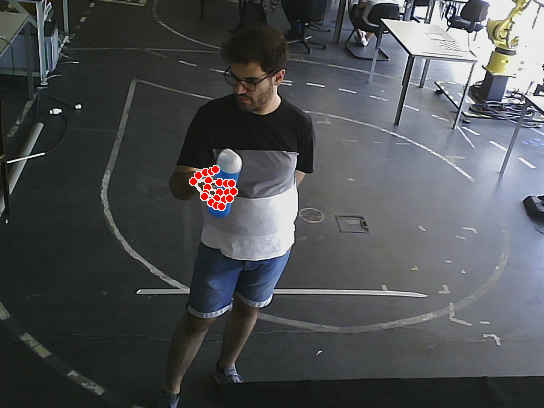
\includegraphics[width=.9\textwidth]{figs/dataset_preprocessing2_1.png}}} (body_keypoints)
                (body_keypoints) edge node[right] {right hand keypoints} (normalization) 
                (normalization) edge node[above] {normalized right hand keypoints} (model)
                (model) edge (output)
                ;

    \if{0}
    \node [rblock] (camera) {Camera\\Image};
    \node [block, right =0.5cm of camera] (hands_keypoints) {Mediapipe\\Hands\\Model};
    \node [block, right =0.5cm of hands_keypoints] (body_keypoints) {Mediapipe\\Full Body\\Model};
    \node [block, right =0.5cm of body_keypoints] (normalization) {Points\\Normalization};
    \node [block, right =0.5cm of normalization] (model) {Model\\Prediction};
    \node [rblock, right =0.5cm of model] (output) {Predicted\\Object};

    %% paths
    \path[draw,->, text width=1.7cm, align=center]
                (camera) edge (hands_keypoints)
                (camera) edge[bend right] (body_keypoints)
                (hands_keypoints) edge (body_keypoints)
                (body_keypoints) edge (normalization) 
                (normalization) edge (model)
                (model) edge (output)
                ;
    \fi
    
\end{tikzpicture}
    \caption{Machine Learning Pipeline}
    \label{fig:ml_pipeline}
\end{figure}


\section{Data Collecting}

The first step to train a supervised machine learning model is to find a dataset. However, given that this problem is very specific the datasets had to be manually collected. For this purpose, 2 datasets were collected with both consisting of a set of videos where one person would be moving and rotating a certain object. These videos were recorded at 10 frames per second to avoid consecutive frames having similar hand poses.

\begin{figure}[H]
\centerline{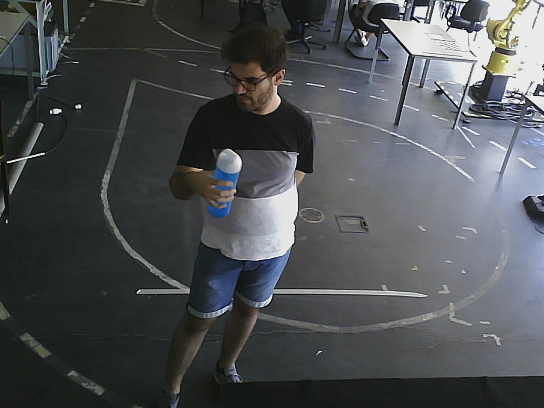
\includegraphics[width=0.49\textwidth]{figs/dataset_preprocessing1_1.png} 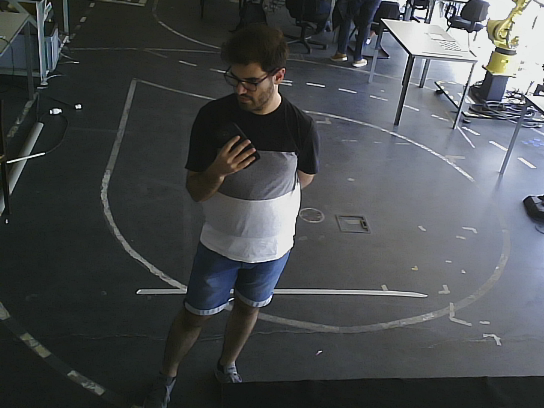
\includegraphics[width=0.49\textwidth]{figs/dataset_preprocessing1_2.png}}
\caption[Dataset Examples]{Dataset Examples}
\label{fig:dataset_examples}
\end{figure}

In the first dataset, 3 different objects were used (see Fig: x), and for each one, 1 person was recorded for 30 seconds resulting in 300 images per object. In the second dataset, 4 objects were used (see Fig: x), and 3 people were recorded in 4 different 25-second videos for each object resulting in 1000 frames for each person and object making it 3000 frames for each object. Recording more than one video for each combination of person and object allowed each person to grasp the object slightly differently each time in order to obtain a more diverse dataset.

\textcolor{red}{image with objects}

\section{Dataset Preprocessing}

After having a dataset, the data had to be processed so that it would have a fitting structure to be used in the model training and testing. The images from the videos were processed using the Mediapipe hands model resulting in 21 points for each hand detected. The images were also processed by the full-body model also provided by Mediapipe so that it is possible to identify the right hand.

\begin{figure}[H]
\centerline{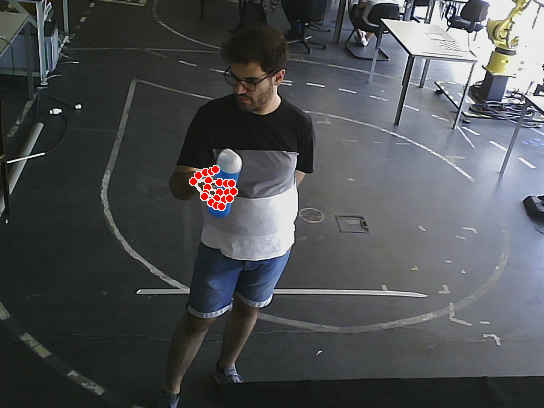
\includegraphics[width=0.49\textwidth]{figs/dataset_preprocessing2_1.png} 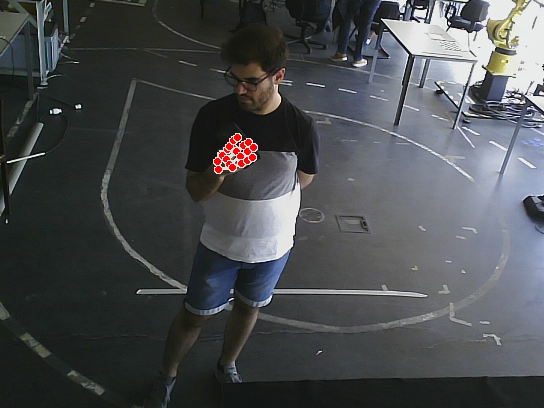
\includegraphics[width=0.49\textwidth]{figs/dataset_preprocessing2_2.png}}
\caption[Dataset Examples]{Dataset Examples}
\label{fig:dataset_examples}
\end{figure}

These points are then subject to further processing and normalization so that the location of the hand in the image and the distance between the hand and the camera have a lesser impact. The centroid is calculated and the points are translated so that they are centered in the (0.5, 0.5, 0.5) point, the points are then scaled up as much as possible while keeping every coordinate of every point between 0 and 1.

\begin{figure}[H]
\centerline{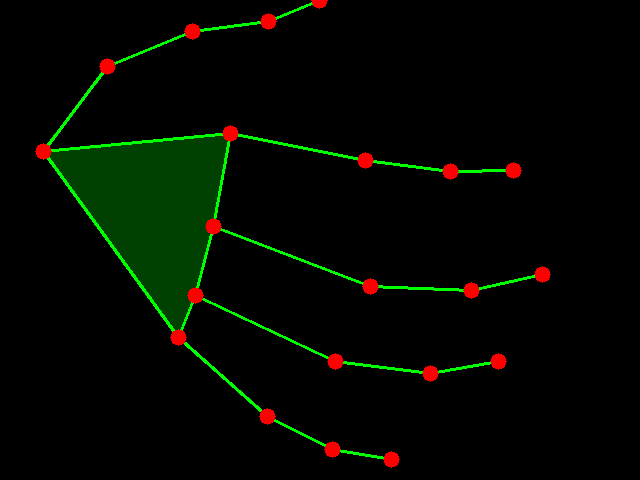
\includegraphics[width=0.49\textwidth]{figs/dataset_preprocessing3_1.png} 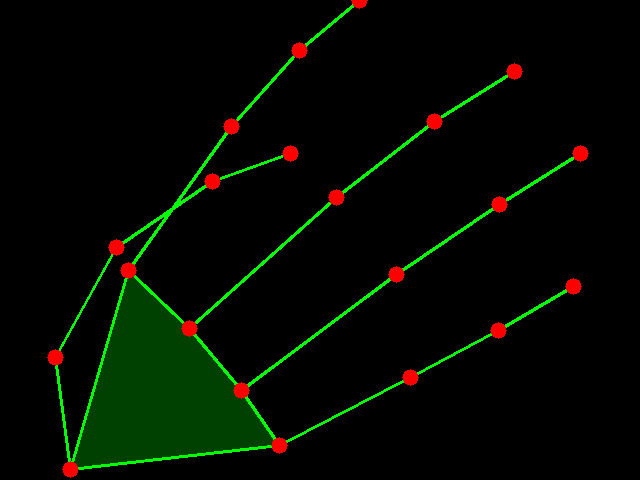
\includegraphics[width=0.49\textwidth]{figs/dataset_preprocessing3_2.png}}
\caption[Dataset Examples]{Dataset Examples}
\label{fig:dataset_examples}
\end{figure}

\section{Data Splitting}

In order to train the model, the dataset was split into 3 sets: the train set (60\%), the validation set (20\%), and the test set (20\%). The random variables in the data shuffling and splitting were also fixed so that the test set is always the same, and therefore, its data is never used to train or validate the model, even in different trains. During hyperparameter optimization, the different combinations are tested using 4-fold cross-validation, which means that the model is trained 4 times, and therefore every sample of data in the initial training and validation set was used both for training and validation. Additionally, early stopping was set up so that the model would stop after 200 epochs without a better validation loss.

\section{Models}

\subsection{Convolutional Neural Network}

After all the processing, each sample provided to the model is made of the 21 points that represent the right hand. Given that points are related to each other, a one-dimensional convolutional neural network was used to take advantage of this characteristic. Therefore, the CNN is responsible for taking the 21 3D points and classifying the object that is being grasped.

\subsubsection{Initial Results}

Initially, a simple CNN was tested and manually optimized with the first dataset resulting in the following results:

\begin{minipage}{0.35\textwidth}
    \captionof{table}{CNN Results in the First Dataset}
    \label{table:cnn_dataset1_results}
    \centering
    \begin{tabular}{ |p{3.4cm}|p{1.1cm}| }
    \hline
    Metric & Value \\
    \hline
    Training Accuracy & 0.9813 \\
    \hline
    Validation Accuracy & 0.9775 \\
    \hline
    Test Accuracy & 0.9551 \\
    \hline
    Training Loss & 0.0493 \\
    \hline
    Validation Loss & 0.0794 \\
    \hline
    Test Loss & 0.1600 \\
    \hline
    Precision & 0.9583 \\
    \hline
    Recall & 0.9551 \\
    \hline
    F1-Score & 0.9549 \\
    \hline
    \end{tabular}
\end{minipage}%
\begin{minipage}{0.65\textwidth}
    \centering
    \includesvg[width=\textwidth]{figs/cnn_dataset1_conf_matrix.svg}
    %\def\svgwidth{\columnwidth}
    %\input{figs/cnn_dataset1_conf_matrix.pdf_tex}
    \captionof{figure}[CNN Confusion Matrix in the First Dataset]{CNN Confusion Matrix in the First Dataset}
    \label{fig:cnn_confusion_matrix}
\end{minipage}

\kern 0.1cm

Even with a relatively small dataset, this CNN shows positive results with accuracies over 95\%, so it was decided that this model should be tested in the second dataset.

\subsubsection{Final Model Architecture}

When training a model with the initial architecture in the second dataset, the results were considerably lower than those achieved with the first dataset. Given that not only the dataset was bigger, but there was also one more class, it was decided that the model should have a more complex architecture, and with manual optimizations a new architecture was created which had better results. The new model can be seen on Fig.~\ref{fig:cnn_architecture} and it is made of 2 convolutional layers followed by 3 dense layers, with the third being the output layer. Between the convolutional and the dense layers and between both dense layers there is also a dropout layer so as to help with overfitting.

\begin{figure}[H]%[!ht]
    \centering
    \begin{tikzpicture}[>=latex']
    \tikzset{block/.style= {draw, rectangle, align=center,minimum height=2.5cm, scale=1.2},
    rblock/.style={draw, shape=rectangle,rounded corners=1.5em,align=center,minimum width=2cm,minimum height=1cm},
    input/.style={ % requires library shapes.geometric
    draw,
    trapezium,
    trapezium left angle=60,
    trapezium right angle=120,
    minimum width=2cm,
    align=center,
    minimum height=1cm
    },
    }
    
    \node [block] (inputlayer) {\rotatebox{90}{InputLayer}};
    \node [block, right=0.5cm of inputlayer] (conv1d_1) {\rotatebox{90}{Conv1D}};
    \node [block, right=0.5cm of conv1d_1] (conv1d_2) {\rotatebox{90}{Conv1D}};
    \node [block, right=0.5cm of conv1d_2] (flatten) {\rotatebox{90}{Flatten}};
    \node [block, right=0.5cm of flatten] (dropout_1) {\rotatebox{90}{Dropout}};
    \node [block, right=0.5cm of dropout_1] (dense_1) {\rotatebox{90}{Dense}};
    \node [block, right=0.5cm of dense_1] (dropout_2) {\rotatebox{90}{Dropout}};
    \node [block, right=0.5cm of dropout_2] (dense_2) {\rotatebox{90}{Dense}};
    \node [block, right=0.5cm of dense_2] (dense_3) {\rotatebox{90}{Dense}};

    %% paths
    \path[draw,->, text width=3cm, align=center]
                (inputlayer) edge (conv1d_1)
                (conv1d_1) edge (conv1d_2)
                (conv1d_2) edge (flatten)
                (flatten) edge (dropout_1)
                (dropout_1) edge (dense_1)
                (dense_1) edge (dropout_2)
                (dropout_2) edge (dense_2)
                (dense_2) edge (dense_3)
                ;
    
\end{tikzpicture}
    \caption[CNN Architecture]{CNN Model Architecture}
    \label{fig:cnn_architecture}
\end{figure}

%\begin{figure}[H]
%\centerline{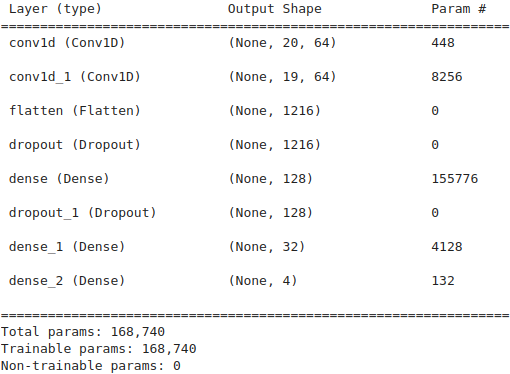
\includegraphics[height=3.4in]{figs/cnn_architecture.png}}
%\caption[CNN Architecture]{CNN Model Architecture}
%\label{fig:cnn_architecture}
%\end{figure}

\subsubsection{Hyperparameter Optimization}

In this model, 3 common hyperparameters in CNNs were optimized to obtain better results. These were the initial learning rate for the model training, the kernel size used by the convolutional layers and the dropout rate. Additionally, the number of convolutional layers was also tested given that, according to manual testing, it also affected the model results without changing the number of trainable parameters. The values tested for each hyperparameter can be seen on Table \ref{table:cnn_hyperparameters}.

\begin{table}[H]
\caption{Tested Hyperparameter Values}
\label{table:cnn_hyperparameters}
\centering
\begin{tabular}{|l|l|}
\hline
Hyperparameter & Tested Values \\
\hline
Learning Rate & 0.01, 0.001, 0.0001 \\
\hline
Number of Convolutional Layers & 1, 2, 3 \\
\hline
Kernel Size & 2, 3 \\
\hline
Dropout Rate & 0.0, 0.1, 0.2, 0.3, 0.4, 0.5 \\
\hline
\end{tabular}
\end{table}

In order to choose the best combination of these hyperparameters, all combinations were tested using 4-fold cross validation, which means that the model was trained 4 times, and every sample of data was used both for training and validation. It is important to note that the process to obtain these hyperparameters did not include the data from the test set. Then the average result of each combination was obtained with the combination in Table \ref{table:cnn_best_hyperparameters} having the lowest average loss with 0.2100 and an average accuracy of 94.20\%.

\begin{table}[H]
\captionof{table}{CNN Best Hyperparameters}
\label{table:cnn_best_hyperparameters}
\centering
\begin{tabular}{|l|l|}
\hline
Hyperparameter & Value \\
\hline
Learning Rate & 0.001 \\
\hline
Dropout & 0.5 \\
\hline
Kernel Size & 3 \\
\hline
Number of Convolutional Layers & 2 \\
\hline
\end{tabular}
\end{table}

\subsubsection{Final Results}

With the final architecture defined as well as the model hyperparameters, the final model was trained with the data of the second dataset. The Fig.~\ref{fig:cnn_loss} and Fig.~\ref{fig:cnn_acc} show the evolution of the training and validation loss and accuracy respectively during the training. According to the figures, the best validation loss occurred slightly after the 400th epoch with training stopping 200 epochs later.

% using pretex=\scriptsize reduces all fonts size
\begin{figure}[H]
\centerline{\includesvg[width=\textwidth, pretex=\scriptsize]{figs/cnn_loss_comparison.svg}}
\caption[CNN training and validation loss evolution during training]{CNN training and validation loss evolution during training}
\label{fig:cnn_loss}
\end{figure}

\begin{figure}[H]
\centerline{\includesvg[width=\textwidth, pretex=\scriptsize]{figs/cnn_acc_comparison.svg}}
\caption[CNN training and validation accuracy evolution during training]{CNN training and validation accuracy evolution during training}
\label{fig:cnn_acc}
\end{figure}

With training completed, the metrics in the Table \ref{table:cnn_dataset2_results} were obtained. Given that the validation and test accuracies are close to each other we can conclude that the model managed to generalize its knowledge from the training data to classify data it has never seen before. Additionally, the confusion matrix in the Fig.~\ref{fig:cnn_confusion_matrix} shows that the screwdriver was the object that the model managed to predict more accurately. This can be due to the fact that the hand geometry that allows a person to grasp a screwdriver intuitively is more restrict.

\begin{minipage}{0.35\textwidth}
    \captionof{table}{CNN Results in the Second Dataset}
    \label{table:cnn_dataset2_results}
    \centering
    \begin{tabular}{ |p{3.4cm}|p{1.1cm}| }
    \hline
    Metric & Value \\
    \hline
    Training Accuracy & 0.9601 \\
    \hline
    Validation Accuracy & 0.9442 \\
    \hline
    Test Accuracy & 0.9400 \\
    \hline
    Training Loss & 0.1191 \\
    \hline
    Validation Loss & 0.2171 \\
    \hline
    Test Loss & 0.2291 \\
    \hline
    Precision & 0.9403 \\
    \hline
    Recall & 0.9400 \\
    \hline
    F1-Score & 0.9400 \\
    \hline
    \end{tabular}
\end{minipage}%
\begin{minipage}{0.65\textwidth}
    \centering
    \includesvg[width=\textwidth]{figs/cnn_conf_matrix.svg}
    \captionof{figure}[CNN confusion matrix]{CNN confusion matrix}
    \label{fig:cnn_confusion_matrix}
\end{minipage}

\subsection{Transformer Neural Network}

As said in Subsection \ref{subsection:transformer_neural_networks}, Transformer Neural Networks shine at capturing long-range dependencies and relationships. Therefore, considering the fact that the points obtained from Mediapipe have a specific order, we can take advantage of this ability to process structured data and effectively capture dependencies and patterns.

\subsubsection{Initial Results}

Initially, a Transformer architecture from \textcolor{red}{link} was tested and manually optimized with the first dataset resulting in the following results:

\begin{minipage}{0.35\textwidth}
    \captionof{table}{Tranformer Results in the First Dataset}
    \label{table:transformer_dataset1_results}
    \centering
    \begin{tabular}{ |p{3.4cm}|p{1.1cm}| }
    \hline
    Metric & Value \\
    \hline
    Training Accuracy & 0.8820 \\
    \hline
    Validation Accuracy & 0.8989 \\
    \hline
    Test Accuracy & 0.8820 \\
    \hline
    Training Loss & 0.2794 \\
    \hline
    Validation Loss & 0.2926 \\
    \hline
    Test Loss & 0.3600 \\
    \hline
    Precision & 0.9081 \\
    \hline
    Recall & 0.8820 \\
    \hline
    F1-Score & 0.8835 \\
    \hline
    \end{tabular}
\end{minipage}%
\begin{minipage}{0.65\textwidth}
    \centering
    \includesvg[width=\textwidth]{figs/transformer_dataset1_conf_matrix.svg}
    %\def\svgwidth{\columnwidth}
    %\input{figs/cnn_dataset1_conf_matrix.pdf_tex}
    \captionof{figure}[Transformer Confusion Matrix in the First Dataset]{Transformer Confusion Matrix in the First Dataset}
    \label{fig:transformer_confusion_matrix}
\end{minipage}

\kern 0.1cm

Even with a relatively small dataset, this Transformer shows positive results with accuracies over 88\%. However, when considering the accuracies in each class, we can see that it has greater difficulty in distinguishing between two similar objects. Despite this, it was decided that this model should be tested in the second dataset.

\subsubsection{Model Architecture}

\subsubsection{Hyperparameter Optimization}

\begin{table}[H]
\caption{Tested Hyperparameter Values}
\label{table:transformer_hyperparameters}
\centering
\begin{tabular}{|l|l|}
\hline
Hyperparameter & Tested Values\\
\hline
Learning Rate & 0.01, 0.001, 0.0001\\
\hline
Dropout Rate & 0.0, 0.1, 0.2, 0.3, 0.4, 0.5\\
\hline
MLP Dropout Rate & 0.0, 0.1, 0.2, 0.3, 0.4, 0.5\\
\hline
\end{tabular}
\end{table}

In order to choose the best combination of these hyperparameters, all combinations were
tested using 4-fold cross-validation, and the combination with the smallest average validation loss was chosen. This combination can be seen in Table \ref{table:transformer_best_hyperparameters}
having an average loss of 0.2594 and an average accuracy of 92.24\%.

\begin{table}[H]
\captionof{table}{Transformer Best Hyperparameters}
\label{table:transformer_best_hyperparameters}
\centering
\begin{tabular}{|l|l|}
\hline
Hyperparameter & Value \\
\hline
Learning Rate & 0.0001 \\
\hline
Dropout Rate & 0.5 \\
\hline
MLP Dropout Rate & 0.1 \\
\hline
\end{tabular}
\end{table}

\subsubsection{Final Results}

% using pretex=\scriptsize reduces all fonts size
\begin{figure}[H]
\centerline{\includesvg[width=\textwidth, pretex=\scriptsize]{figs/transformer_loss_comparison.svg}}
\caption[Transformer training and validation loss evolution during training]{Transformer training and validation loss evolution during training}
\label{fig:transformer_loss}
\end{figure}

\begin{figure}[H]
\centerline{\includesvg[width=\textwidth, pretex=\scriptsize]{figs/transformer_acc_comparison.svg}}
\caption[Transformer training and validation accuracy evolution during training]{Transformer training and validation accuracy evolution during training}
\label{fig:transformer_acc}
\end{figure}

\begin{minipage}{0.35\textwidth}
    \captionof{table}{Transformer Results in the Second Dataset}
    \label{table:transformer_dataset2_results}
    \centering
    \begin{tabular}{ |p{3.4cm}|p{1.1cm}| }
    \hline
    Metric & Value\\
    \hline
    Training Accuracy &  0.9414\\
    \hline
    Validation Accuracy & 0.9263\\
    \hline
    Test Accuracy & 0.9244\\
    \hline
    Training Loss & 0.1675\\
    \hline
    Validation Loss & 0.2830\\
    \hline
    Test Loss & 0.2404\\
    \hline
    Precision & 0.9244\\
    \hline
    Recall & 0.9244\\
    \hline
    F1-Score & 0.9243\\
    \hline
    \end{tabular}
\end{minipage}%
\begin{minipage}{0.65\textwidth}
    \centering
    \includesvg[width=\textwidth]{figs/transformer_conf_matrix.svg}
    \captionof{figure}[Transformer confusion matrix]{Transformer confusion matrix}
    \label{fig:transformer_confusion_matrix}
\end{minipage}

\section{Models Comparison}

\begin{table}[H]
\caption{Results with data from one user}
\label{table:results_one_user}
\centering
\begin{tabular}{|l|l|l|l|l|l|l|l|l|} 
\hline
& \multicolumn{4}{|l|}{Loss} & \multicolumn{4}{|l|}{Accuracy} \\
\hline
Model & P1 & P2 & P3 & AVG & P1 & P2 & P3 & AVG \\
\hline
CNN & 0.1897 & 0.3179 & 0.2758 & 0.2611 & 0.9673 & 0.9243 & 0.9378 & 0.9431 \\
\hline
Transformer & \_ & \_ & \_ & \_ & \_ & \_ & \_ & \_ \\
\hline
\end{tabular}
\end{table}

\begin{table}[H]
\caption{Results with a different test user in relation to training}
\label{table:results_2vs1_user}
\centering
\begin{tabular}{|l|l|l|l|l|l|l|l|l|} 
\hline
& \multicolumn{4}{|l|}{Loss} & \multicolumn{4}{|l|}{Accuracy} \\
\hline
Model & P1 & P2 & P3 & AVG & P1 & P2 & P3 & AVG \\
\hline
CNN & 0.6625 & 2.1951 & 1.8477 & 1.5684 & 0.7958 & 0.5970 & 0.5417 & 0.6448 \\
\hline
Transformer & \_ & \_ & \_ & \_ & \_ & \_ & \_ & \_ \\
\hline
\end{tabular}
\end{table}

\section{\textcolor{red}{Integration with Previous Work}}
\chapter{Results and Discussion}
\label{chapter:results_and_discussion}

\chapter{Conclusion \textcolor{red}{and Future Work}}
\label{chapter:conclusion}

This document presented the problem of anticipating human actions in collaborative environments with the goal of developing an anticipatory robot controller for an assembly task. Looking at previous work found in the literature, there is a clear predominance of perception using RGB cameras with different ways of preprocessing the captured images. When it comes to the methods, \acl{ml} and, in particular, supervised learning techniques are predominant, given that most work nowadays takes advantage of the progress made in that field. With the continuous evolution of \acs{ml}, it is expected that the algorithms related to the topic in this paper also evolve and, consequently, give rise to even better solutions. 

To complete the study of previous work, some relevant tools were reviewed with a particular emphasis on two libraries that can detect key points in an image, such as skeleton joints which are very important to detect human poses. Regarding the practical side of the dissertation, an inertial sensor was tested in other to evaluate its inclusion as another source of data. Although it was possible to capture data, an additional effort will be required to demonstrate its usefulness for the proposed study. Furthermore, as a result of this work, the tasks for the second semester were delineated and scheduled.

In summary, the results of this study demonstrate that Action Anticipation is still a relatively new concept, but it has much potential to increase the efficiency and safety of collaborative tasks, revolutionizing the world of \acl{hrc}.

%%%%%%%%%%%%%%%%%%%%%%%%%%%%%%%%%%%%%%%%%%%%%%%%%%%%%%%
% End of Thesis text 
%%%%%%%%%%%%%%%%%%%%%%%%%%%%%%%%%%%%%%%%%%%%%%%%%%%%%%%

\backmatter

%%%%%%%%%%%%%%%%%%%%%%%%%%%%%%%%%%%%%%%%%%%%%%%%%%%%%%%
% Print all used references
%%%%%%%%%%%%%%%%%%%%%%%%%%%%%%%%%%%%%%%%%%%%%%%%%%%%%%%

%\nocite{*}

\begingroup
\renewcommand{\bibfont}{\footnotesize}
% Redefine References name to Portuguese
% Change if you are using english
\defbibheading{bibliography}[References]{
	\chapter{#1}
}
\SingleSpacing
\setlength\bibitemsep{8pt}
\printbibliography[heading=bibliography]
\endgroup


%%%%%%%%%%%%%%%%%%%%%%%%%%%%%%%%%%%%%%%%%%%%%%%%%%%%%%%
% Load appendix
%%%%%%%%%%%%%%%%%%%%%%%%%%%%%%%%%%%%%%%%%%%%%%%%%%%%%%%

\mainmatterWithoutReset
\appendix

% \include{appendix-a}
% \include{appendix-b}
% \include{appendix-c}

\end{document}
